\section{Preface}
\textit{The following chapter extends the idea of energy minimisation principles introduced by the Tsigankov-Koulakov model used in the previous chapter. It aims to use this idea to generate a model which offers the same explanatory power of experimental data while posing the problem in such a way that it can be computed efficiently and with natural interpretations. This would help solve the significant computational challenges experienced with using the Tsigankov-Koulakov model at large scales. The chapter focuses first on detailing the model, demonstrating performance increases, and explaining several well-known phenotypes.}

\section{Introduction}
As discussed in Section \ref{sec:models}, models of retinotopic mapping have developed to the stage where they can largely reproduce the phenomenology of various mutants by sufficient manipulation of their parameters. While this is encouraging for scientific explanation and prediction, the parameter manipulation presents a significant challenge to model assessment and interpretability. As an example consider a model of an organism calibrated to a wild-type $W$ with parameter set $\vec{Q}$ which can explain mutants $A$ and $B$ which arise from seemingly independent mechanisms, say Hebbian plasticity and chemotaxis, with parameter sets $\vec{Q_A}$ and $\vec{Q_B}$. If the parameters sets differ to the wild-type only with respect to the mechanisms which they claim to explain then it the model is likely to be sound. In the more likely case, where these parameters changes are intermingled between mechanisms, there is a significant interpretability problem: do these mechanisms regulate each other, or was the wild-type calibrated incorrectly? If the mechanisms regulate each other then the model has made a strong experimental prediction: it suggests an unexpected and falsifiable effect. If the parameters are not robust and need recalibration for every new data-set it suggests over fitting which dramatically reduces the predictive power and explainability of the model especially considering many of them are universal function generators. The question is then how do we quantitatively discriminate between competing models?

A recent review of current models proposed the following methodology: first calibrate the model parameters to the example that allows for the most parsimonious explanation of the data, next vary mutant specific parameters, and finally select the model which made the best quantitative predictions \cite{Hjorth2015-le}. The model which quantitatively accounts for the most data under this method is the Tsigankov-Koulakov model \cite{Tsigankov2006-uy, Triplett2011-jk}. The essential feature of the Tsigankov-Koulakov model was incorporating all the relevant mechanisms into a linearly independent energy functional. The minimised functional represents the final organised state of the map i.e. the functional contains information about the mechanisms guiding development but not the time course of development itself. Mechanisms such as chemotaxis, activity correlation structures, and competition can then be incorporated; see Section \ref{section:developmentaltheory} \cite{Seabrook2017-fa, Lemke2005-iz, Triplett2011-jk, Cang2013-dw}. This procedure is effective because the mechanistic effects of these actions have been incorporated into the functional definition itself. This energy based functional approach is useful because other mechanisms can be added or removed as needed. For example, it has been argued that fibre-fibre interactions are an essential feature of topographic organisation, and this can be added once the mechanistic endpoint can be expressed as a locally convex minimisation problem with respect to the synaptic connections \cite{Weth2014-dq}. 

There are a few key issues with the Tsigankov-Koulakov model which are all inter-related: developmental time-course interpretation, computational complexity, and a lack of understanding of the parameter space. The interpretation of time is difficult because the model uses a stochastic minimisation procedure similar to a Metropolis-Hastings procedure that allows at each simulated time-step for synapses to created and deleted at long distances which would violate physical principles but do not change the local minima of the functional and are therefore mathematically legitimate \cite{William_H_Press2007-kb}. The reason this minimisation procedure is chosen is because it is efficient in high-dimensional spaces: the Tsigankov-Koulakov model is a discrete model from a pre-synaptic space of $n$ neurones to a post-synaptic space of $m$ neurones in which every potential function can be examined yielding a function space of the order $m^n$; the common case being $n=m=10000$. 

The minimisation is CPU bound and, with $n$ retinal/collicular neurons, involve an $O(n^2)$ operations applied at least 1000 times to each retinal cell yielding a minimal computational bound of $o(n^3)$ \cite{Triplett2011-jk}. To reach accurate convergence in the studies performed in Chapter \ref{chapter:lattice} required that each potential synapse, not retinal cell, should be sampled a number of times increasing the bound to $O(n^4)$. For high resolution maps involving comparable numbers of neurones to the real biological system the computational wall time on modern CPU architectures can exceed ~18 hours. To understand the parametric properties of a particular phenotype at even small samples sizes of 100 generated maps we had to downsample the resolution of the model to $n=2000$; a five-fold reduction which decreases the prior confidence we have on effects being real and not model resolution artefacts. A genealogy of parameters now exists in the Tsigankov-Koulakov model as a result of parameter fitting with the most recent prediction suggesting neural activity regulates chemotaxis \cite{Koulakov2004-ia, Tsigankov2006-uy, Tsigankov2010-on, Triplett2011-jk, Lyngholm2019-fs}. The reason that statistical and large-scale parameter studies have not been completed can be largely attributed to computational cost with only one study to date providing a parameter robustness analysis which required the use of a super-computer \cite{Tikidji-Hamburyan2016-sn}.

It is desirable to have a model which encapsulates the same explanatory power of the existing Tsigankov-Koulakov model while formalising the mechanistic issues discussed in Chapter \ref{chapter:review} and decreasing the computational cost to allow for efficient computational studies to be carried out. The focus of this Chapter will be to develop a model, here called ``Distributed Kernels'', which extracts the useful features of the existing class of unified models discussed in Section \ref{sec:models} but which can be easily interpreted and efficiently parallelised on a GPU architecture.
  
\section{Distributed Kernels Model Definition}
The review of existing models suggest that an affinity-based interpretation gradients is likely the only gradient based mechanism which will be able to explain the $Math5^{-/-}$ mutant. This is most efficiently encoded in terms of an energy functional following the approach by Tsigankov and Koulakov (2006) to define a developed retinotopic map $w$ by the minimiser of a functional $E$ parametrised by a parameter vector $\vec{Q}$ \cite{Tsigankov2006-uy}. This energy functional is composed of linearly independent contributions from various mechanisms:
\begin{equation}
E[w(\vec{x}; \vec{Q})] = \sum_{u \in \text{mechanisms}} E_u[w(\vec{x}; \vec{Q})],
\end{equation}
where the mechanisms are arbitrarily defined according to the appropriate data. Currently available data suggest that the three mechanisms of chemotaxis, correlated activity, and competition are sufficient to explain retinotopic maps developmental endpoints and these are incorporated into the model. With a locally convex curvature a gradient descent based scheme would allow a natural interpretation of developmental time allowing time to be incorporated in an energy based approach in a principled manner. It is then a matter of appropriately encoding each mechanisms energy contribution to mimic the developmental dynamics of the system.
\subsection{Representation of Physical Structures}
Encoding the physical representation of the problem helps to specify initial conditions and to interpret the data. In a population of $N$ retinal cells each cell is modelled as a discrete unit $i$ which is associated with a function or kernel that is a function of position in the collicular space. 

This kernel can be interpreted as either a series of synaptic weights or as a probability distribution. A natural way to represent the function associated with retinal cell $i$ is by a Gaussian kernel density estimator:
\begin{equation}\label{eq:probkernels}
p_i(\vec{x}) = \frac{1}{\sigma M \sqrt{2 \pi}}\sum_{j=1}^{M} \exp\left(-\frac{\left|\vec{x} - \vec{x}^i_j\right|^2}{2\sigma^2}\right),
\end{equation}
where $j$ indexes the series representation of the synaptic distribution of the retinal cell $i$, $\vec{x}_j$ represents the colliculus location at which the Gaussian associated with $j$ is centred; see Figure \ref{fig:kernelexample}. The probability distribution interpretation allows a natural mapping back into the discrete space of the colliculus: at the endpoint sample each distribution $m$ times according to how many synaptic contacts the retinal neurone is expected to make and attach each of these to the colliculus cell which is locally most dominant. The number of synaptic contacts may be allowed to vary between retinal cells, but it is assumed not to, and local dominance will be measured by Euclidean distance. The modelling of afferents in this fashion allows for calculations of the synaptic kernel to be easily distributed amongst many processes making parallelisation simple: this is the root of the model name.
\begin{figure}[h]
	\centering
	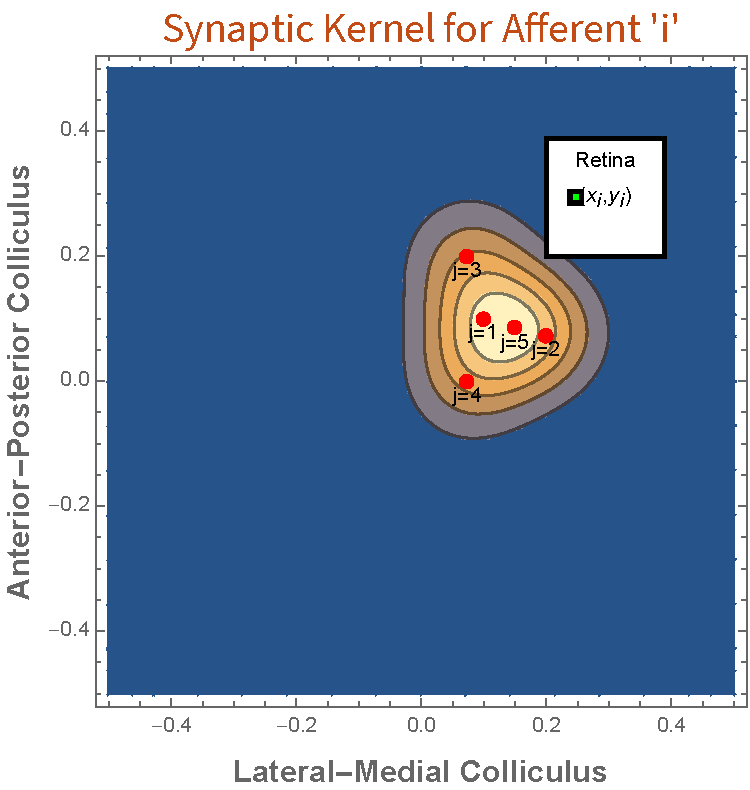
\includegraphics[width=0.75\textwidth]{images/distributed_kernels/figure_kernelexample}
	\def\c{An example of a potential probability distribution of synpatic contacts for a given retinal afferent.}
	\caption[\c]{\label{fig:kernelexample} The synaptic kernel for a single retinal afferent $i$ at retinal location $(x_i, x_j)$ shown in green. The kernel is composed of the linear combination of five Gaussian kernels; see Equation \ref{eq:probkernels}. The Gaussian kernels are centred at $\{\vec{x}_j\}_{j=1}^5$ and these are shown as red dots labelled by $j \in \{1, ..., 5\}$. The total synaptic kernel is composed of the linear combination of the kernels for each retinal afferent $i \in \{1, ..., N \}$.}
\end{figure}
A useful first-order simplification is to let $\sigma\rightarrow0$ supposing that each retinal afferents synaptic distribution is composed of a series of Dirac-Delta functions. This simplification confers three advantages. It simplifies the algebraic integrations, is computationally efficient, and allows the model to be thought of as the dynamics of a series of discrete points associated with the retinal afferents; this interpretation makes it similar to the Simpson-Goodhill model \cite{Simpson2011-zh} and is a useful and natural mental model.

The geometry of both the retina and the colliculus is taken to be the unit circle. This choice is made for simplicity and does not make a substantial computational difference for the reasons discussed in Section \ref{section:autodifferentiation}.
\subsection{Mechanisms}
The mechanisms are formulated by associating each mechanism with an energy functional and assuming linear independence to combine them into a total functional. While this energy functional, in principle, can be extended to incorporate all relevant mechanisms this work will focus on the three major mechanisms: chemotaxis, activity, and competition. 
\begin{equation}
E[w(\vec{x}; \vec{Q})] = E_\text{chem}[w(\vec{x}; \vec{Q})]  + E_\text{act}[w(\vec{x}; \vec{Q})]  + E_\text{comp}[w(\vec{x}; \vec{Q})],
\end{equation}
where $w(\vec{x}; \vec{Q}) = \sum_i p_i(\vec{x}; \vec{q_i} \in \vec{Q})$ is the total collection of all retinal inputs and $\vec{Q}$ is the collection of parameter vectors $\vec{q}_i$ which define the location and size of each kernel distribution in $p_i$. With an analytical expression for $E[w(\vec{x}; \vec{Q})]$ the problem amounts to adequate minimisation of the expression on its parameter space. As discussed in Section \ref{sec:minimisation} there are many schemes for minimizing a function some of which have convergence guarantees but it is noted that there is no known general method to find a global minima. 

Gradient descent is a local optimisation scheme which is proven to converge to a local minima provided the function is locally convex which will follow for each of the components of the energy function. This makes it a desirable choice for the problem and reduces it to computing $\nabla_{\vec{Q}}E[w(\vec{x}; \vec{Q})]$. Gradient descent schemes can be accelerated by a variety of momentum based methods and this work uses the ADAM optimiser with the default parameters $\alpha = 0.99$, and $\beta = 0.999$  \cite{kingma2017adam}. 

Each functional needs to be detailed to arrive at expressions for the gradient descent scheme. These can be fed into a standard implementation of the ADAM optimiser and compiled into GPU code. This will be performed using the Julia language in conjunction with CUDA.
\subsection{Chemotaxis}
The chemotactic energy follows directly from the law of mass action being proportional to the product of the expression level of Eph receptor and ephrin ligand. Labelling the retinal coordinates by $(x_i, y_i)$ the expression levels by the symbol $X_Z^Y(x, y)$ where $X \in \{R, L\}$ denotes a receptor or ligand, $ Y \in \{r, c\}$ denotes the retina or the colliculus, and $Z \in \{A, B\}$ denotes the A and B subsystems respectively. The local chemotactic energy will be directly proportional to the amount of interacting ligands and receptors in a given area determined by the local concentration in the colliculus and the proportional contributions added by the synaptic kernel of each afferent. The total chemotactic energy will be the integral over the entire domain of the colliculus, $\mathcal{D}$, of each of these local contributions:
\begin{align} \label{eq:chemotaticenergy}
	E_\text{chem}[w(x, y), x, y] = &\sum_i \int_{\mathcal{D}} p_i(x, y) (\alpha(R^c_A(x)L^r_A(x_i) + R^r_A(x_i)L^c(x)) \\ - &\beta(R^c_B(y)L^r_A(y_i) + R^r_B(y_i)L^c(y)))dxdy.
\end{align}
Let $R^c_A(x) = \exp(0.5 - x)$, $L^c_A(x) = \exp(x - 0.5), R^r_A(x) = 2\exp(0.5 - x)$, $L^r_A(x) = \exp(x - 0.5),  R^c_B(y) = \exp(0.5 - y)$, $L^c_B(y) = \exp(y - 0.5), R^r_B(y) = 2\exp(0.5 - y)$, $L^r_B(y) = \exp(y - 0.5)$; see Figure \ref{fig:cartoongradients}. These gradients represent the simplest exponential gradient profile in Eph and ephrin expression levels and are chosen for simplicity over the complex but more scientifically accurate profiles examined in the previous chapter. There is no substantive difference for the purposes of this work but the more accurate profiles should be used when making quantitative predictions. These gradients and the definitions for the kernels given by equation \ref{eq:probkernels} are inserted into equation \ref{eq:chemotaticenergy} to arrive at the expression for chemotactic energy. 
\begin{figure}[h]
	\centering
	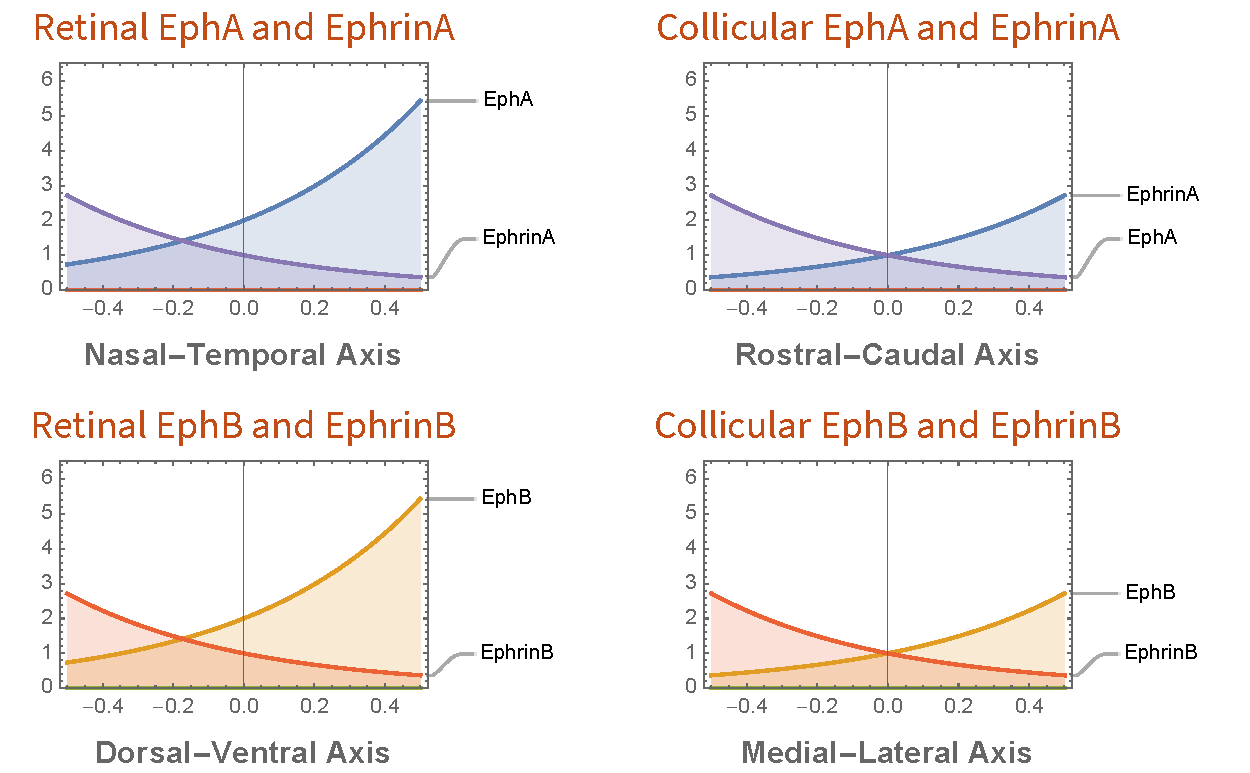
\includegraphics[width=0.75\textwidth]{images/distributed_kernels/figure_cartoongradients}
	\def\c{The gradients and counter-gradients used for the A and B systems in the retina and colliculus. }
	\caption[\c]{\label{fig:cartoongradients} \c These gradients are combined as a single masked gradient which results in the model implementing a Type I graded matching chemotactic mechanism; see Section \ref{sec:chemotaxismodelling}.}
\end{figure}
\subsection{Neural Activity}
The neural activity based energy will be a function of the product of the correlation between activity levels on each pair of synapses in the target. The correlation structures arise as a function of the complex spatio-temporal patterns of the waves and the Hebbian rule under which synapse modification operates. These modifications can be precisely calculated to inform a prior in the correlation structure of each pair of synapses by following the work detailed in Chapter \ref{chapter:neuralstdp}. It is assumed, for simplicity, that there is a isotropic distance dependent correlation function in both the retina and colliculus of the form $C^Y(\vec{x}, \vec{y}; \vec{A}_Y)  = a_1\exp\left(-\frac{\left| \vec{x} - \vec{y}\right|^2}{2 a_2^2}\right)$ where $Y \in \{r,c\}$ denotes the retina or colliculus and $\vec{A}_Y$ is a vector containing the parameters defining the correlation. The activity energy contribution at an infinitesimal location $(x,y)$ in the colliculus is given by the convolution of all of the synaptic kernels multiplied by the correlation between functions between them:
\begin{equation} \label{eq:activityenergy}
dE_\text{act}(x, y) = \gamma \sum_i \sum_j \int_{\mathcal{D}} p_i(x_i - s, y_i - t)p_j(x, y) C^c(x - s, y - t)C^r(S_r(i, j)) ds dt,
\end{equation}
where $S_r(i,j)$ is the distance in the retina between the $i$'th and the $j$'th neuron. The total activity energy is simply the integral of the local energy over the entire colliculus domain $\mathcal{D}$:
\begin{equation}
E_\text{act} = \gamma \sum_i \sum_j \int_{\mathcal{D}} \int_{\mathcal{D}}p_i(x_i - s, y_i - t)p_j(x_j-x,y_j-y) C^c(s -x, t - y; \vec{Q}_c))C^r(S_r(i, j); \vec{Q}_r) ds dt dx dy.
\end{equation}
Again, these and the definitions for the kernels given by equation \ref{eq:probkernels} in the Dirac-Delta limit are inserted into equation \ref{eq:activityenergy} to arrive at the expression for activity energy.
\subsection{Competition}
Each pair of afferents $i$ and $j$ will attempt to compete for resources in the colliculus and this demand will be bound by a local neighbourhood $P$ in colliculus space which is assumed to decay exponentially with the square of the distance and parametrised by $\eta$: $P(x,y; \eta) = \exp(-(x^2+y^2)/(2\eta)^2)$. Therefore, the competitive energy will be defined by integrating this local neighbourhood kernel against every pair of afferents over the the colliculus domain:
\begin{equation}
\label{eq:compenergy}
E_\text{comp} = \gamma \sum_i \sum_j \int_{\mathcal{D}} \int_{\mathcal{D}}p_i(x_i - s, y_i - t)p_j(x_j-x,y_j-y) P(x,y; \eta) ds dt dx dy .
\end{equation}
Again, these and the definitions for the kernels given by equation \ref{eq:probkernels} in the Dirac-Delta limit are inserted into equation \ref{eq:compenergy} to arrive at the expression for the competitive energy.
\subsection{Delayed Competition and Neural Activity Activation}
The mouse retinotopic system undergoes chemotactic signalling before the waves of neural activity are presented; see Chapter \ref{chapter:biology}. To capture this in the model the energy term was restricted to just the chemotactic component for the first 1/5 of the development time. After this time the other mechanisms were instantiated.
\subsection{Generating the Kernel}
To generate the kernel it is assumed that each retinal neurone can metabolically support up to a given number of synapses. The probability distribution of each neurone defines how to sample these synapses. This choice is somewhat arbitrary and does not take into account colliculus demand for resources.  However, the competition mechanism should be sufficient to capture most competitive interactions in the colliculus. The Dirac-Delta limit was used to generate the probability distribution which presents a problem for sampling as this now defines a categorical rather than continuous distribution. Sampling from this distribution is feasible but it is more natural to think of an area on which synapses can be placed. To achieve this it is assumed that the Dirac-Delta simplification provides a valid approximation for the centres of the Gaussians in the probability distribution and the standard deviation is assumed to be small, in this case 0.001, which then defines a continuous probability distribution for each retinal index. The synapse number was set to ten and the number of kernels to three. 
\subsection{Auto-Differentiation: Efficient Computation of Derivatives} \label{section:autodifferentiation}
Auto-differentiation is a computational method to find the derivative of a function that can be expressed as a series of operations with computational cost proportional to the cost of calling the function \cite{Speelpenning1980-mt, innes2019dont}. This is done by constructing the computational graph of the function and traversing that graph forwards or backwards and collecting derivative operations on each node. This gives a way to calculate the derivative efficiently provided the energy function can be defined computationally. As mentioned earlier, the specific geometries of the retina and the colliculus, and the specific instantiations of the functions in the energy terms should not pose a significant challenge to the run-time operations of the model but a choice must be made such that it can be explicitly evaluated. 

The software package Flux.jl has an implementation of auto-differentiation that works well with functions that have a native Julia implementation \cite{innes2019dont, Flux.jl-2018}. Substantial work has been done to ensure that this routine extends naturally to GPU based functions running in CUDA \cite{innes2018}. There is a performance hit compared to a hard-coded derivative, particularly in memory cost, which can be limiting for GPUs. Nevertheless, it demonstrates the language works flexibly at a high level with fairly minimal performance costs. As such, no efforts are made to optimise the code at the compiler level.
\subsection{Code and System Specifics}
The above considerations can be condensed into several subroutines which formally define the model. These routines are written entirely in native Julia but link to CUDA via the CUDA package. The package dependencies are Random, CUDA, Flux.jl,  and StatsBase. The simulations were performed on a combination of an AMD Ryzen 3950x CPU and Nvidia 3090 GPU. The code base can be found freely available on GitHub \cite{DistributedKernels}. 
\section{Results}
The speed objective demands a demonstrable run-time speed up against the existing Tsigankov-Koulakov model. Therefore, the first study is to compare the wall times of both methods against each other. A single kernel is chosen and the of number of nodes used in the simulation varied to keep the two routines comparable. The run-times up to 4000 nodes are presented in Figure \ref{fig:distributedruntimes}. The linear fit to the log transformed data in both cases is good ($R^2 = 0.999$ and $R^2=0.945$) suggesting that there are well defined scaling properties for each routine. The Koulakov model scales as $N^{3.29}$ and the Distributed Kernels Model scales as $N^{0.94}$.

\begin{figure}[h]
	\centering
	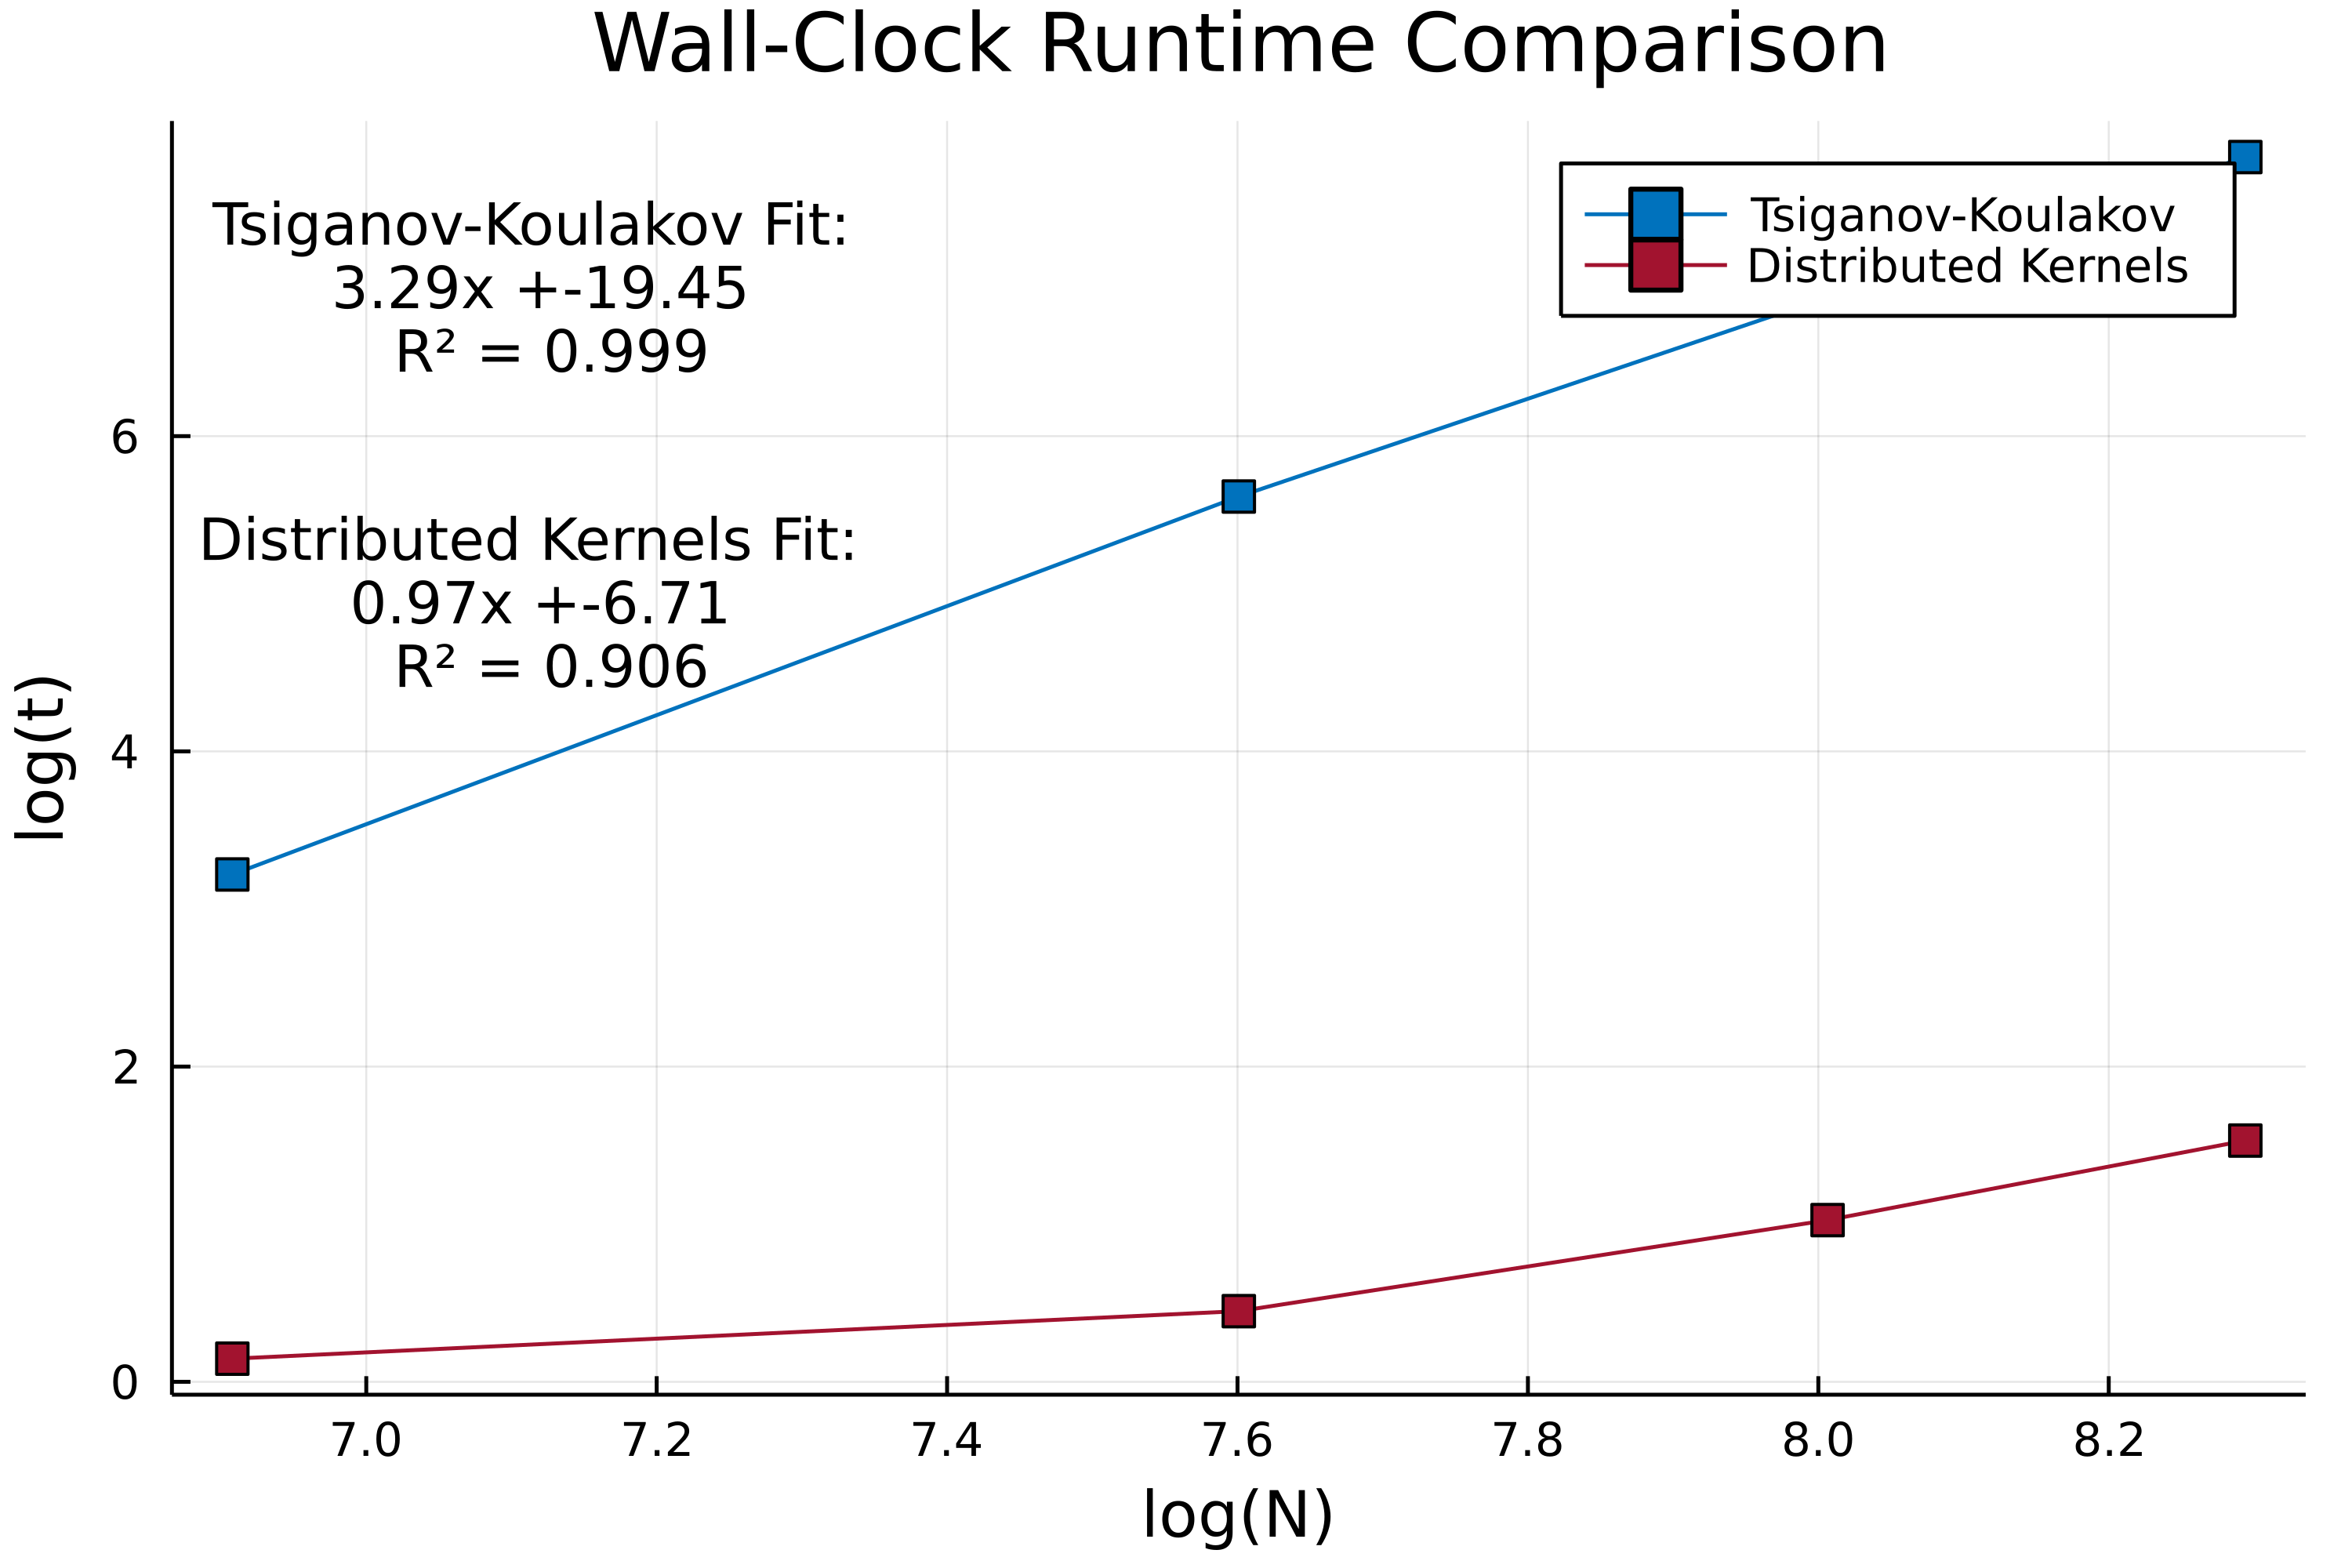
\includegraphics[width=0.75\textwidth]{images/distributed_kernels/figure_runtime}
	\def\c{The log-transformed runtime plots for the Tsigankov-Koulakov and Distributed Kernels models are plotted in blue and red respectively}
	\caption[\c]{\label{fig:distributedruntimes} \c. Time is measured in seconds showing that The fits to the log transformed data are good suggesting well defined scaling laws. The Tsigankov-Koulakov model scales at least as a cubic while the Distributed Kernels model scales slightly less than linear. This sub-linear scaling is expected to slightly increase with higher $N$ as the GPU unit becomes saturated.}
\end{figure}

\subsection{Phenotype Reproduction}
The model must be no less explanatory than the existing models and therefore must be able to replicate the phenomenological descriptions of various mutants. This is demonstrated by analysing four classes which so far only the Tsigankov-Koulakov has been able to correctly model: wild-type, ephrinA2A5 knock-down, EphA3 knock-in, and $Math5^{-/-}$. For each mutant 900 retinal neurones are simulated each with 3 associated Gaussian's; $M = 3$ in Equation \ref{eq:probkernels}. The minimisation procedure is completed in 200 applications of the ADAM optimiser and 10 samples from each retinal cell distribution are taken to form the topographic map for a total of 27000 contacts. This number is comparable to the 10000 synaptic contacts formed in the Tsigankov-Koulakov model. Similarity to previous results is demonstrated in two key ways: a simulated series of coloured injections corresponding to a rainbow map across the retina, and forward and reverse lattice plots. The rainbow plot smoothly assigns each retinal location a unique colour and all of that locations synaptic contacts accordingly inherit this colour.

\subsubsection{Wild-Type}
The wild type phenotype is simulated by choosing $\alpha = 1, \beta = 1, \gamma = -0.05, \delta = 0.3, s = 0.075$. These parameters are subsequently fixed in all future simulations unless the phenotype demands that they change to maintain modelling consistency. The rainbow plot is displayed in Figure \ref{fig:wtrainbow} and shows a visually smooth continuous association between the pre-synaptic and post-synaptic regions. There is a detectable jitter corresponding to retinal locations having overlapping arbours in the SC. The forward (field to colliculus) and reverse (colliculus to field) lattice plots are shown in Figure \ref{fig:wtlattice}. Both of these plots demonstrate a continuous and unbiased projection in both directions. The mapping errors are minimal and restricted to the boundaries. The lattice plots are also homogenous showing no clustering or density around any particular region.

\begin{figure}[hbt!]
	\centering
	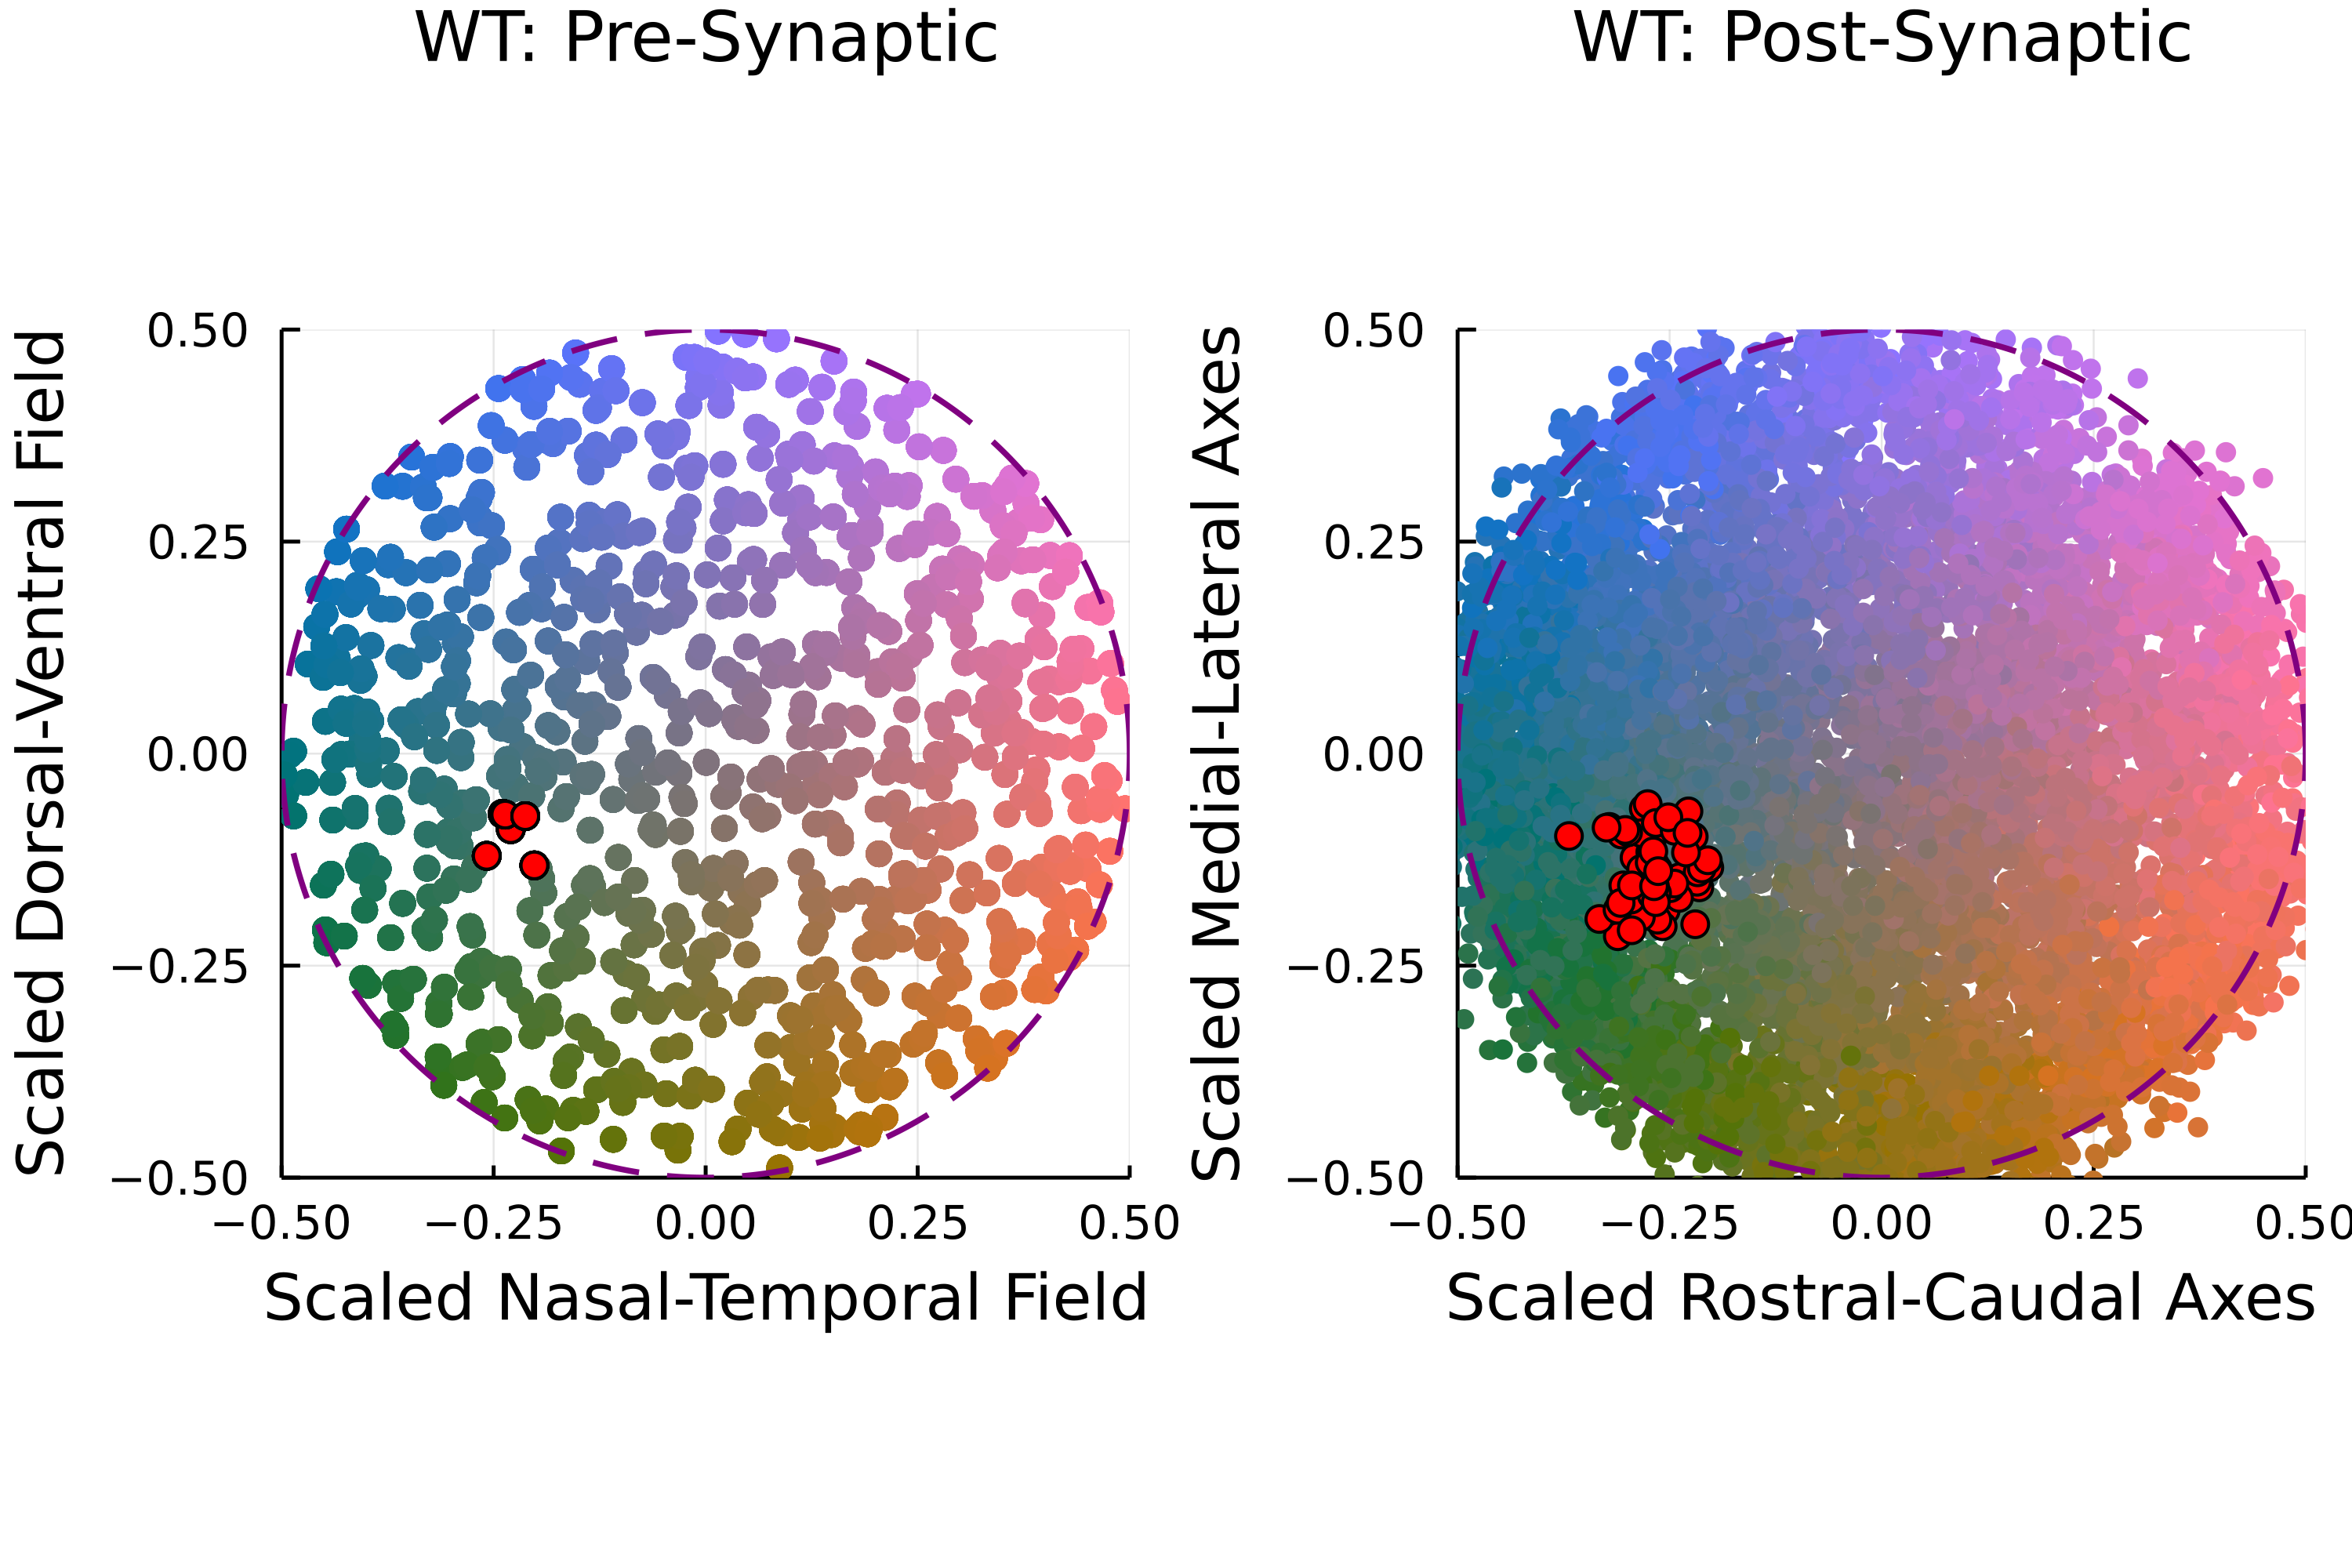
\includegraphics[width=\textwidth]{images/distributed_kernels/figure_distributed_kernels_WT}
	\def\c{A rainbow plot for the wild-type, or calibration, phenotype. Under the choice of a parameters $\alpha = 1, \beta = 1, \gamma = -0.05, \delta = 0.3, s = 0.075$ a smoothly varying topographic map with slightly overlapping topographic arbours is generated. }
	\caption[\c]{\label{fig:wtrainbow} \c A tracer injection experiment is modelled by selecting a 1\% area of the retina and highlighting the region of the colliculus it projects to in red.}
\end{figure}

\begin{figure}[hbt!]
	\centering
	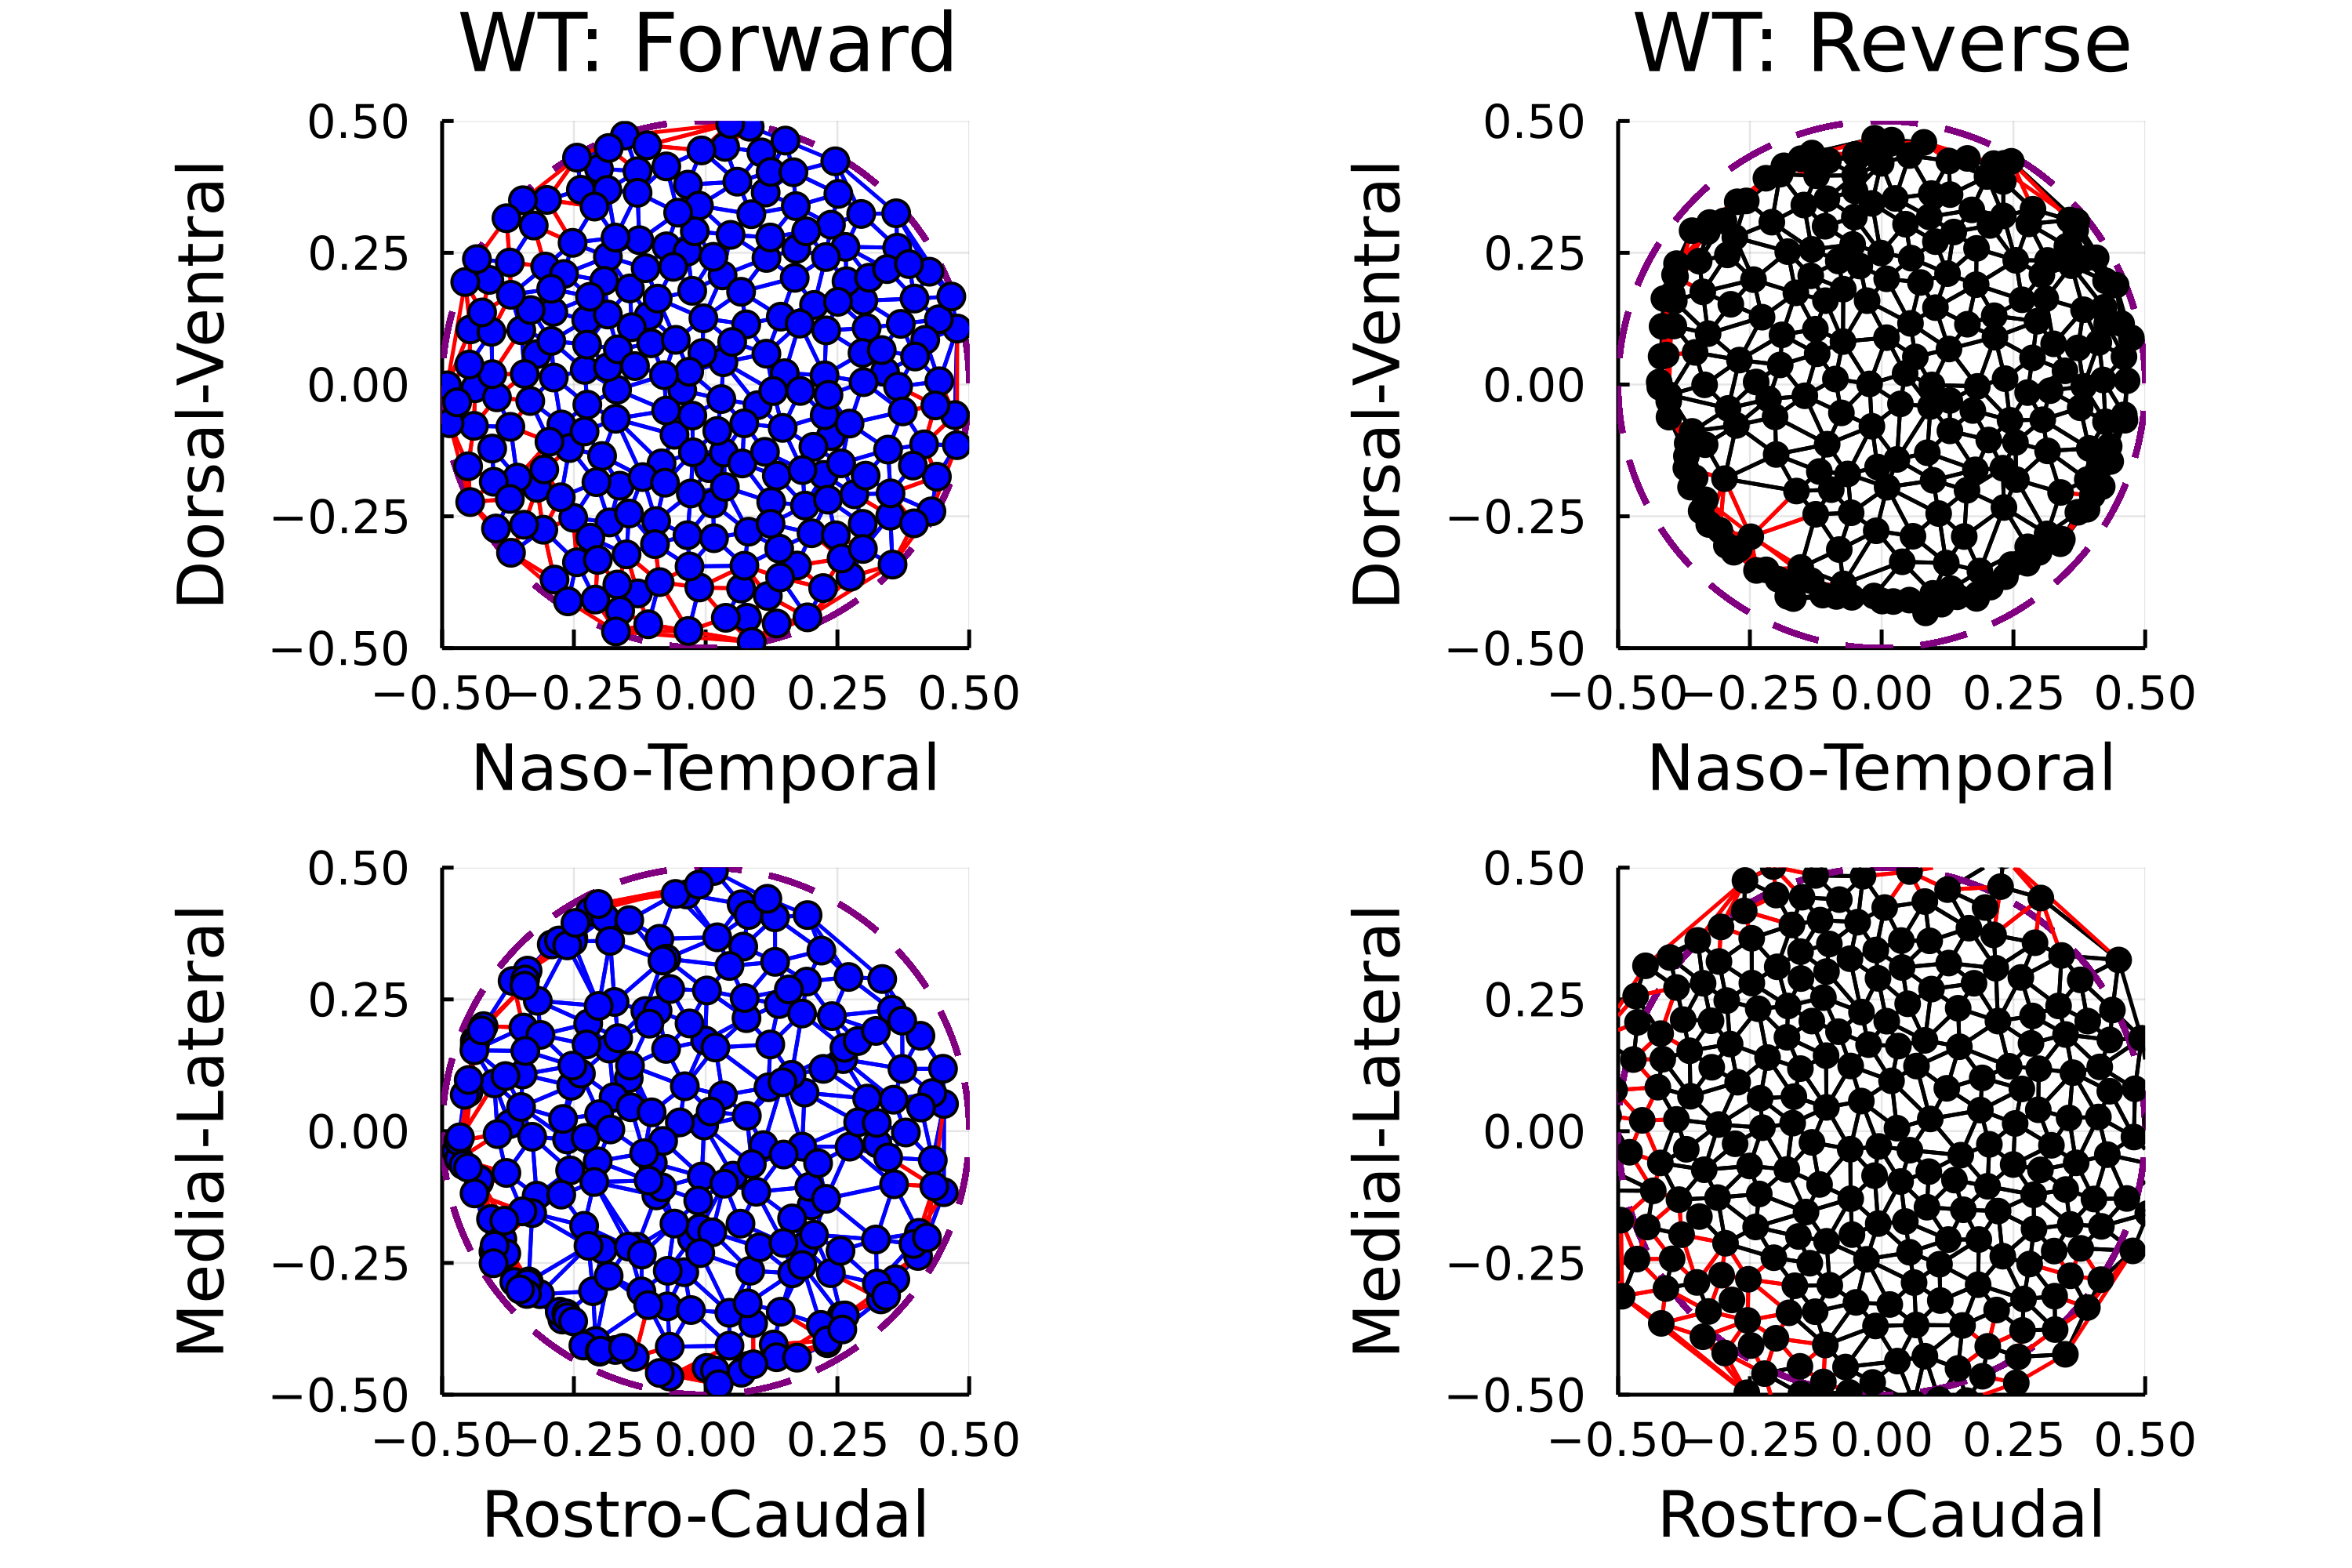
\includegraphics[width=\textwidth]{images/distributed_kernels/figure_lattice_WT}
	\caption{\label{fig:wtlattice} Forward and reverse lattice plots for the wild-type, or calibration, phenotype and are generated in the same fashion as those in Figure \ref{fig:wholemap}. Both projections show a smooth and well-ordered lattice with minimal mapping errors. The spacing is evenly distributed and no region in either of the images has a favourable or dense projection.}
\end{figure}
\newpage
\subsection{ephrinA Triple Knockout}
The ephrinA2A3A5 knockout mutant represents a near complete removal of the ephrinA ligand guidance system and this was simulated by choosing $L_A(x) = 0$ resulting in no chemical energy dependence on one of the axes \cite{Cang2013-dw}. This results in severe topographic mapping errors, particularly along the rostro-caudal axis. The rainbow plot shown in Figure \ref{fig:ephrina2a5_rainbow} shows a complete disordering along the rostro-caudal axis while maintaining visual order along the medial-lateral axes. The retinal injection experiment highlighted in red shows a series of projections throughout the superior colliculus and is comparable to injection experiments performed on a similar mutant: the ephrinA2A5 double knockout \cite{Feldheim2000-be}. The forward lattice plot is compressed to the midline of the rostrocadual axis. The reverse lattice plot is slightly more structured and covers a larger section of the visual field. These are comparable to lattice analysis performed on EphrinA2A3A5 mutants \cite{Willshaw2014-ms}.
\begin{figure}
	\begin{subfigure}{\textwidth}
		\centering
		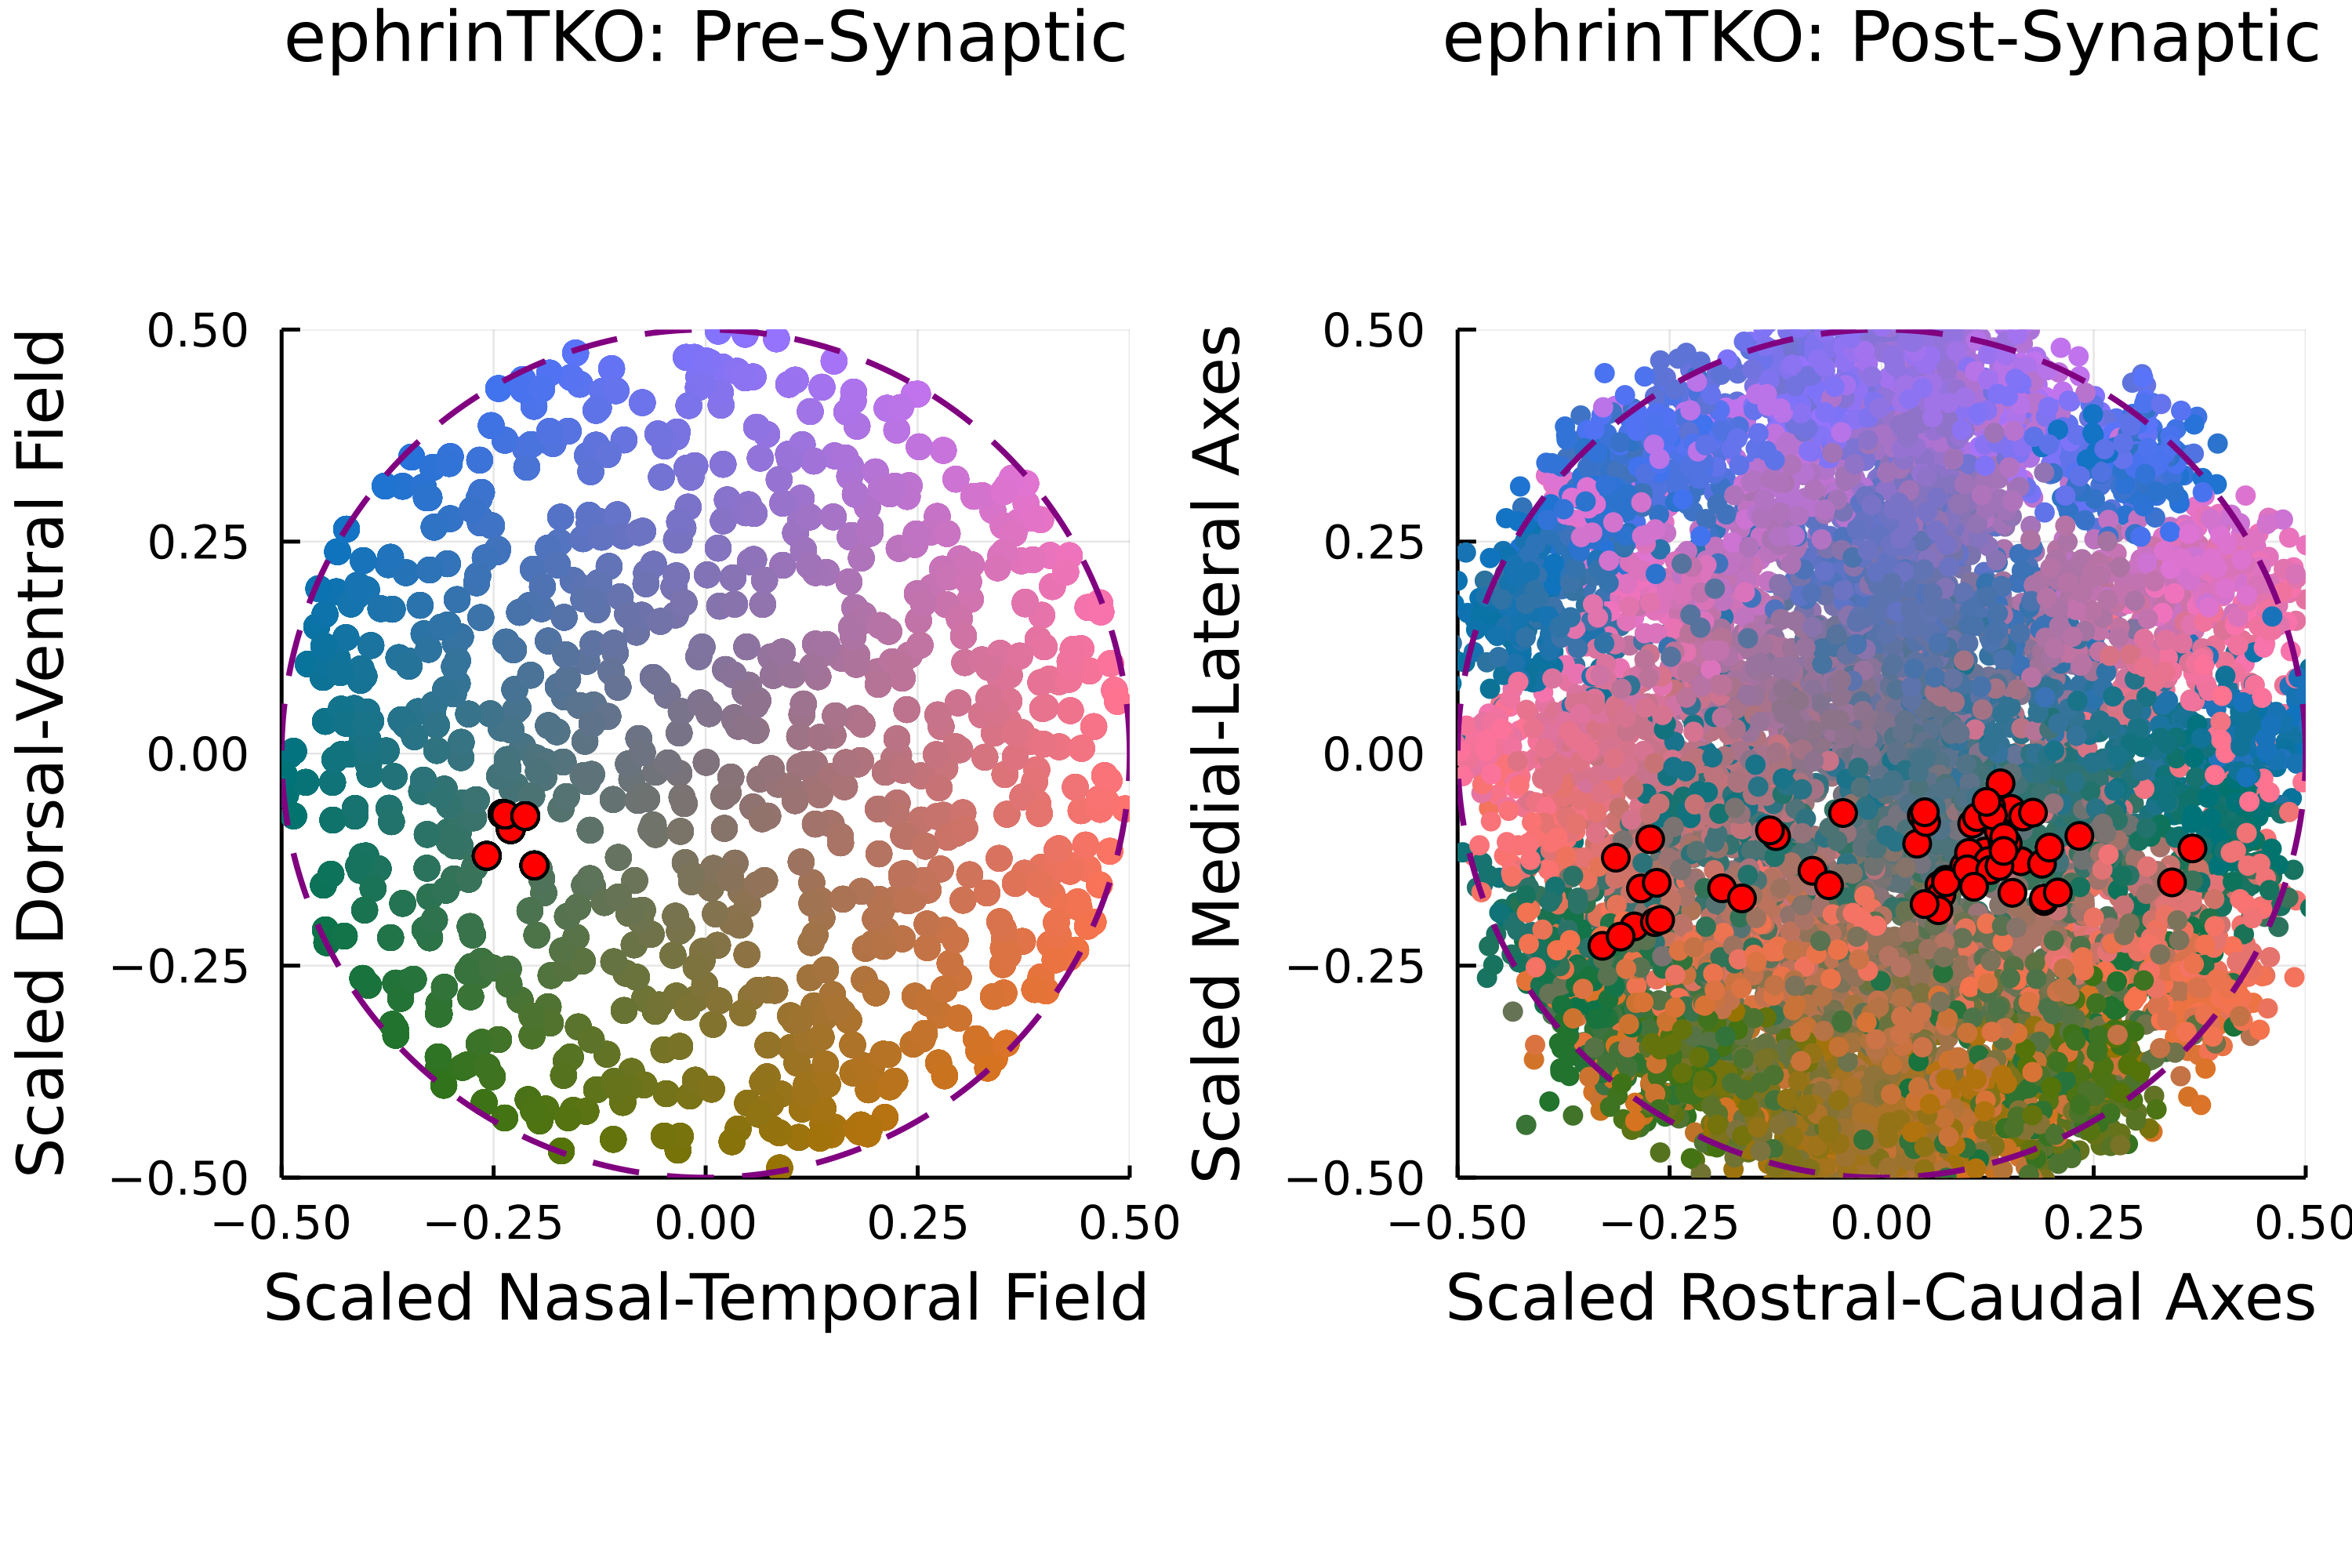
\includegraphics[width=\textwidth]{images/distributed_kernels/figure_distributed_kernels_ephrinTKO}
		\caption{}
	\end{subfigure}
~
	\begin{subfigure}{0.33\textwidth}
	\centering
	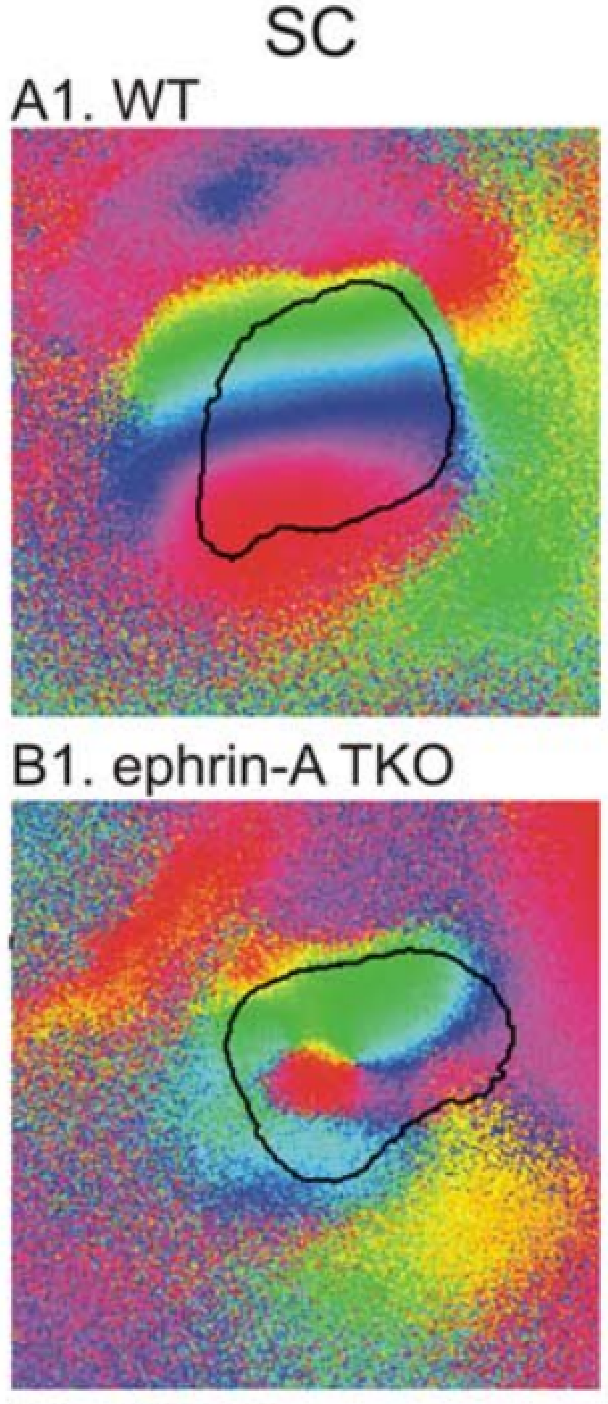
\includegraphics[width=\textwidth]{images/distributed_kernels/ephrinTKOois}
	\caption{}
	\end{subfigure}
\qquad\qquad\qquad\qquad\qquad
	\begin{subfigure}{0.3\textwidth}
		\centering
		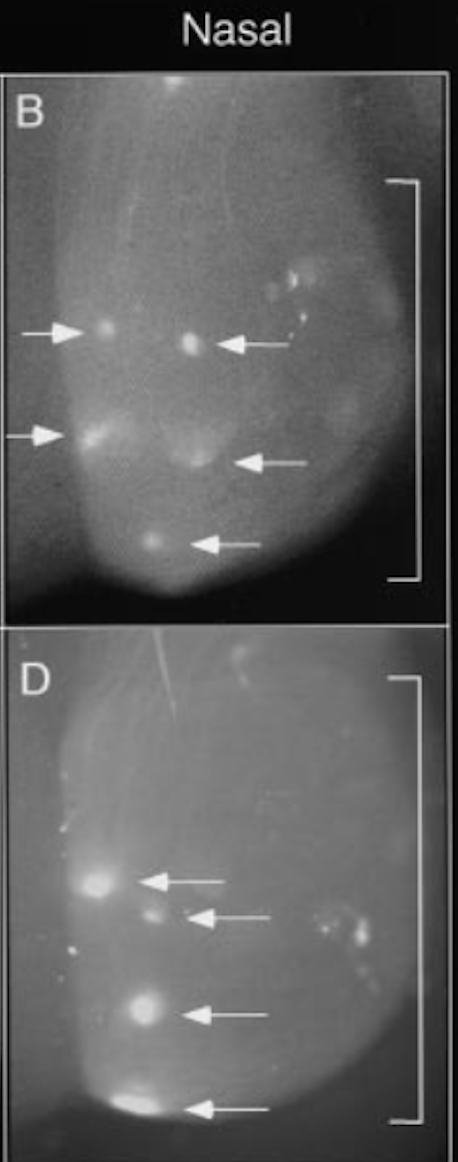
\includegraphics[width=\textwidth]{images/distributed_kernels/ephrinA2A5double}
		\caption{}
	\end{subfigure}
	\def\c{A rainbow plot for the ephrinA-TKO phenotype is presented. }
	\caption[\c]{\label{fig:ephrina2a5_rainbow} A rainbow plot for the ephrinA-TKO phenotype is presented in the top panel (a). A small retinal injection is made in the nasal retina which reveals a wide distribution of anatomical termination zones. Data for genotypes that significantly disrupt ephrinA expression are shown in panel (b) with DiI injections into EphrinA2A5 double knock-out mice shown in the leftmost panels and an azimuthal intrinsic optical imaging scan of an EphrinA2A3A5 triple knock-out shown in the rightmost panel. Figures adapted from Feldheim et. al. (2000) and Cang et. al. (2008) \cite{Feldheim2000-be, Cang2008-ez}. }
\end{figure}

\begin{figure}
	\begin{subfigure}{0.7\textwidth}
		\centering
		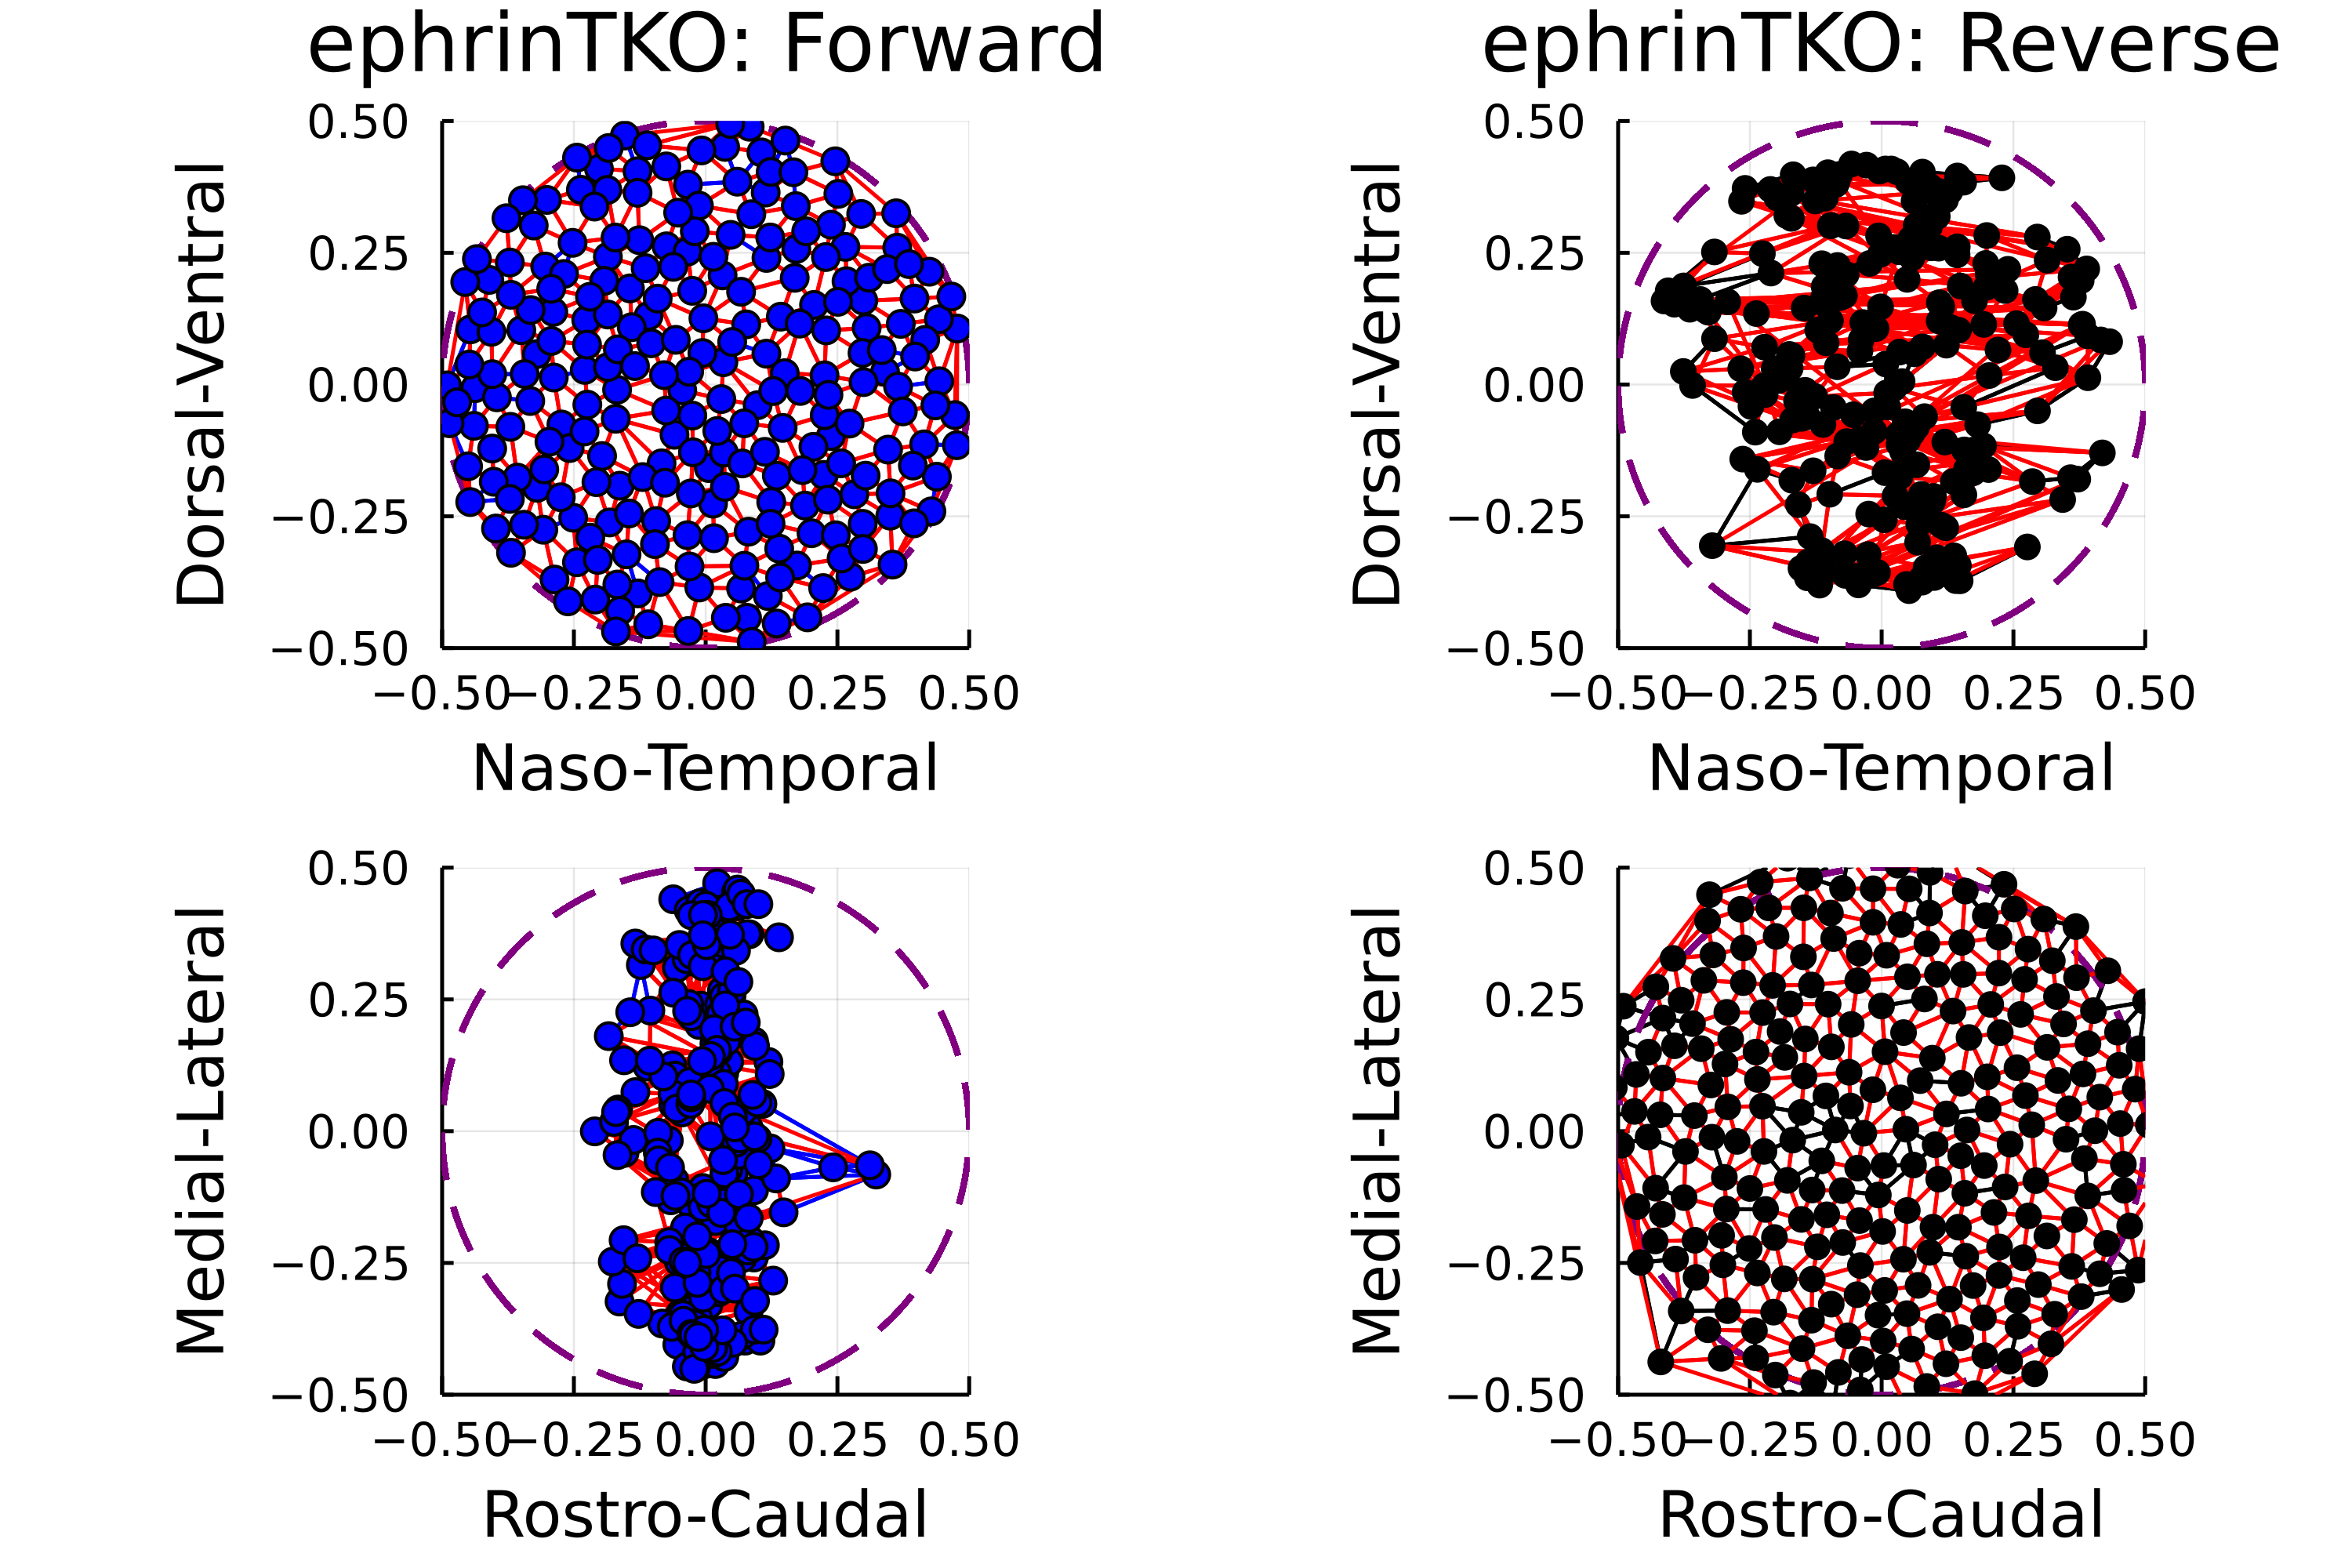
\includegraphics[width=\textwidth]{images/distributed_kernels/figure_lattice_ephrinTKO}
		\caption{}
	\end{subfigure}
~
	\begin{subfigure}{0.26\textwidth}
	\centering
	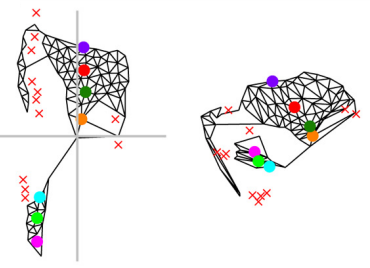
\includegraphics[width=\textwidth]{images/distributed_kernels/latticeephrinTKO}	
	\caption{}
	\end{subfigure}
	\def\c{Forward and reverse lattice plots for the ephrinA-TKO phenotype are presented. }
	\caption[\c]{\label{fig:ephrina2a5_lattice} Forward and reverse lattice plots for the ephrinA-TKO phenotype are presented in panel (a). Both projections demonstrate a notable disorder in the map. The forward plot demonstrates that the nasal-temporal axis is collapsed onto the rostral caudal axis while the dorsal-ventral axes is relatively maintained. The reverse projection highlights that the visual field is still well covered by the colliculus, but the mapping is disordered. This is in line analysis of optical image scanning maps and a sample of a forward map is presented in panel (b) adapted from Willshaw et. al (2014) \cite{Willshaw2014-ms}. The axes convention differs slightly for the experimental data-based map with vertical alignment of the rostral-caudal and nasal-temporal axes. The map compression and corruption along this axes can be seen.}
\end{figure}
\newpage
\subsection{$Math5$ knock-out}
In the $Math5^{-/-}$ mutant only 5\% of retinal cells are born resulting in lower competition between RGCs \cite{Triplett2011-jk}. It highlights the competitive interaction between incoming afferents and its importance for establishing correct topography. Competition was simulated by choosing $\delta = 0.00$ thereby eliminating the competitive energy. The rainbow plot shown in Figure \ref{fig:math5_rainbow} a well ordered cluster of points in a single quadrant of the post-synaptic field. There is no data available for the $Math5^{-/-}$ in terms of the fine structure; the retinal dye flood injection experiment is shown which highlights the colliculus boundary.
\begin{figure}
	\begin{subfigure}{\textwidth}
		\centering
		\includegraphics[width=\textwidth]{images/distributed_kernels/figure_distributed_kernels_math5}
		\caption{\label{fig:math5_rainbow}}
		
	\end{subfigure}
	~
	\begin{subfigure}{0.6\textwidth}
		\centering
		\includegraphics[width=\textwidth]{images/distributed_kernels/figure_lattice_math5}	
		\caption{\label{fig:math5_lattice}}
	\end{subfigure}
		\begin{subfigure}{0.4\textwidth}
		\centering
		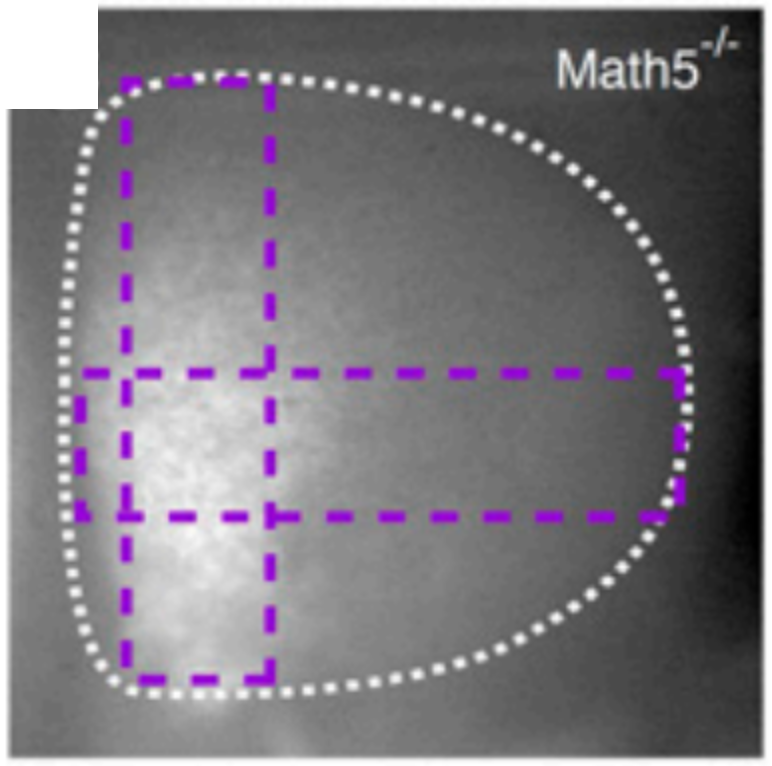
\includegraphics[width=\textwidth]{images/distributed_kernels/math5}	
		\caption{}
	\end{subfigure}
	\def\c{A rainbow plot for the $Math5^{-/-}$ phenotype. }
	\caption[\c]{\c The projection is clustered towards the lower left quadrant corresponding to the rostral-medial region of the colliculus is shown in (a). The projection remains relatively ordered despite the compression but interestingly a retinal injection occupies a simple area as in the wild-type. A whole field injection is shown in (c) which highlights the extent to which the $Math5^{-/-}$ mutant occupies the colliculus; figure adapted from Triplett et. al. (2011) \cite{Triplett2011-jk}. Forward and reverse lattice plots for the $Math5^{-/-}$ phenotype are shown in (b). The forward projection shows a highly concentrated but well ordered map with the density increasing towards the boundary region. The mapping errors increase with proximity to the boundary. The reverse projection maintains a well-ordered structure with a small amount of mapping errors interestingly clustered on the interior boundary.}
\end{figure}


\newpage
\subsection{EphA3 knock-in}
The EphA3 mutant represents an insert of a non-endogenous EphA receptor on the $Islet2$ cassette expressed in approximately 40\% of retinal cells \cite{Brown2000-da, Reber2004-wq}. Both the homozygous and heterozygous forms of this phenotype have been studied and were the subject of the Chapter \ref{chapter:lattice} but here attention is focused on the homozygous form which creates a double map. 

The phenotype is simulated as in Chapter \ref{chapter:lattice} by creating a mask of tagged EphA3 positive cells selected randomly from all available cells with probability 0.4, and increasing the chemical energy provided by the A system on these cells by adding $\Delta R = 0.05$ to the retinal gradient at each of these locations; the transition between the homozygous and heterozygous phenotypes can be found by manipulating this $\Delta R$. The rainbow plot shown in Figure \ref{fig:epha3_rainbow} demonstrate a clear bifurcation of two complete maps with the caudal side occupying slightly less space. The retinal injection shows two anatomical projections highlighting the double map in line with data \cite{Brown2000-da}.

The lattice plots are broken into two subsets: the forward projections are lattices constructed independently using only $Islet2^{+/-}$ cells(and their contacts) or $Islet2^{-/-}$ cells i.e. the EphA3 retinal mosaic and the wild-type mosaic. The reverse projections are created by creating a dividing line at $x = 0.0$ in the post-synaptic region and using only the contacts which satisfy being on one side of this line. They are comparable to the data derived lattice plots from the previous chapter with two maps being revealed with an overlap. The forward plots cannot be associated with any data because current experiments do not highlight the EphA3 specific projection. They are comparable to the forward plots generated by the model in the previous chapter revealing that the EphA3 tagged cells are compressed into the caudal region while the wild-type cells tend to project over the whole colliculus.

\begin{figure}
	\begin{subfigure}{\textwidth}
		\centering
		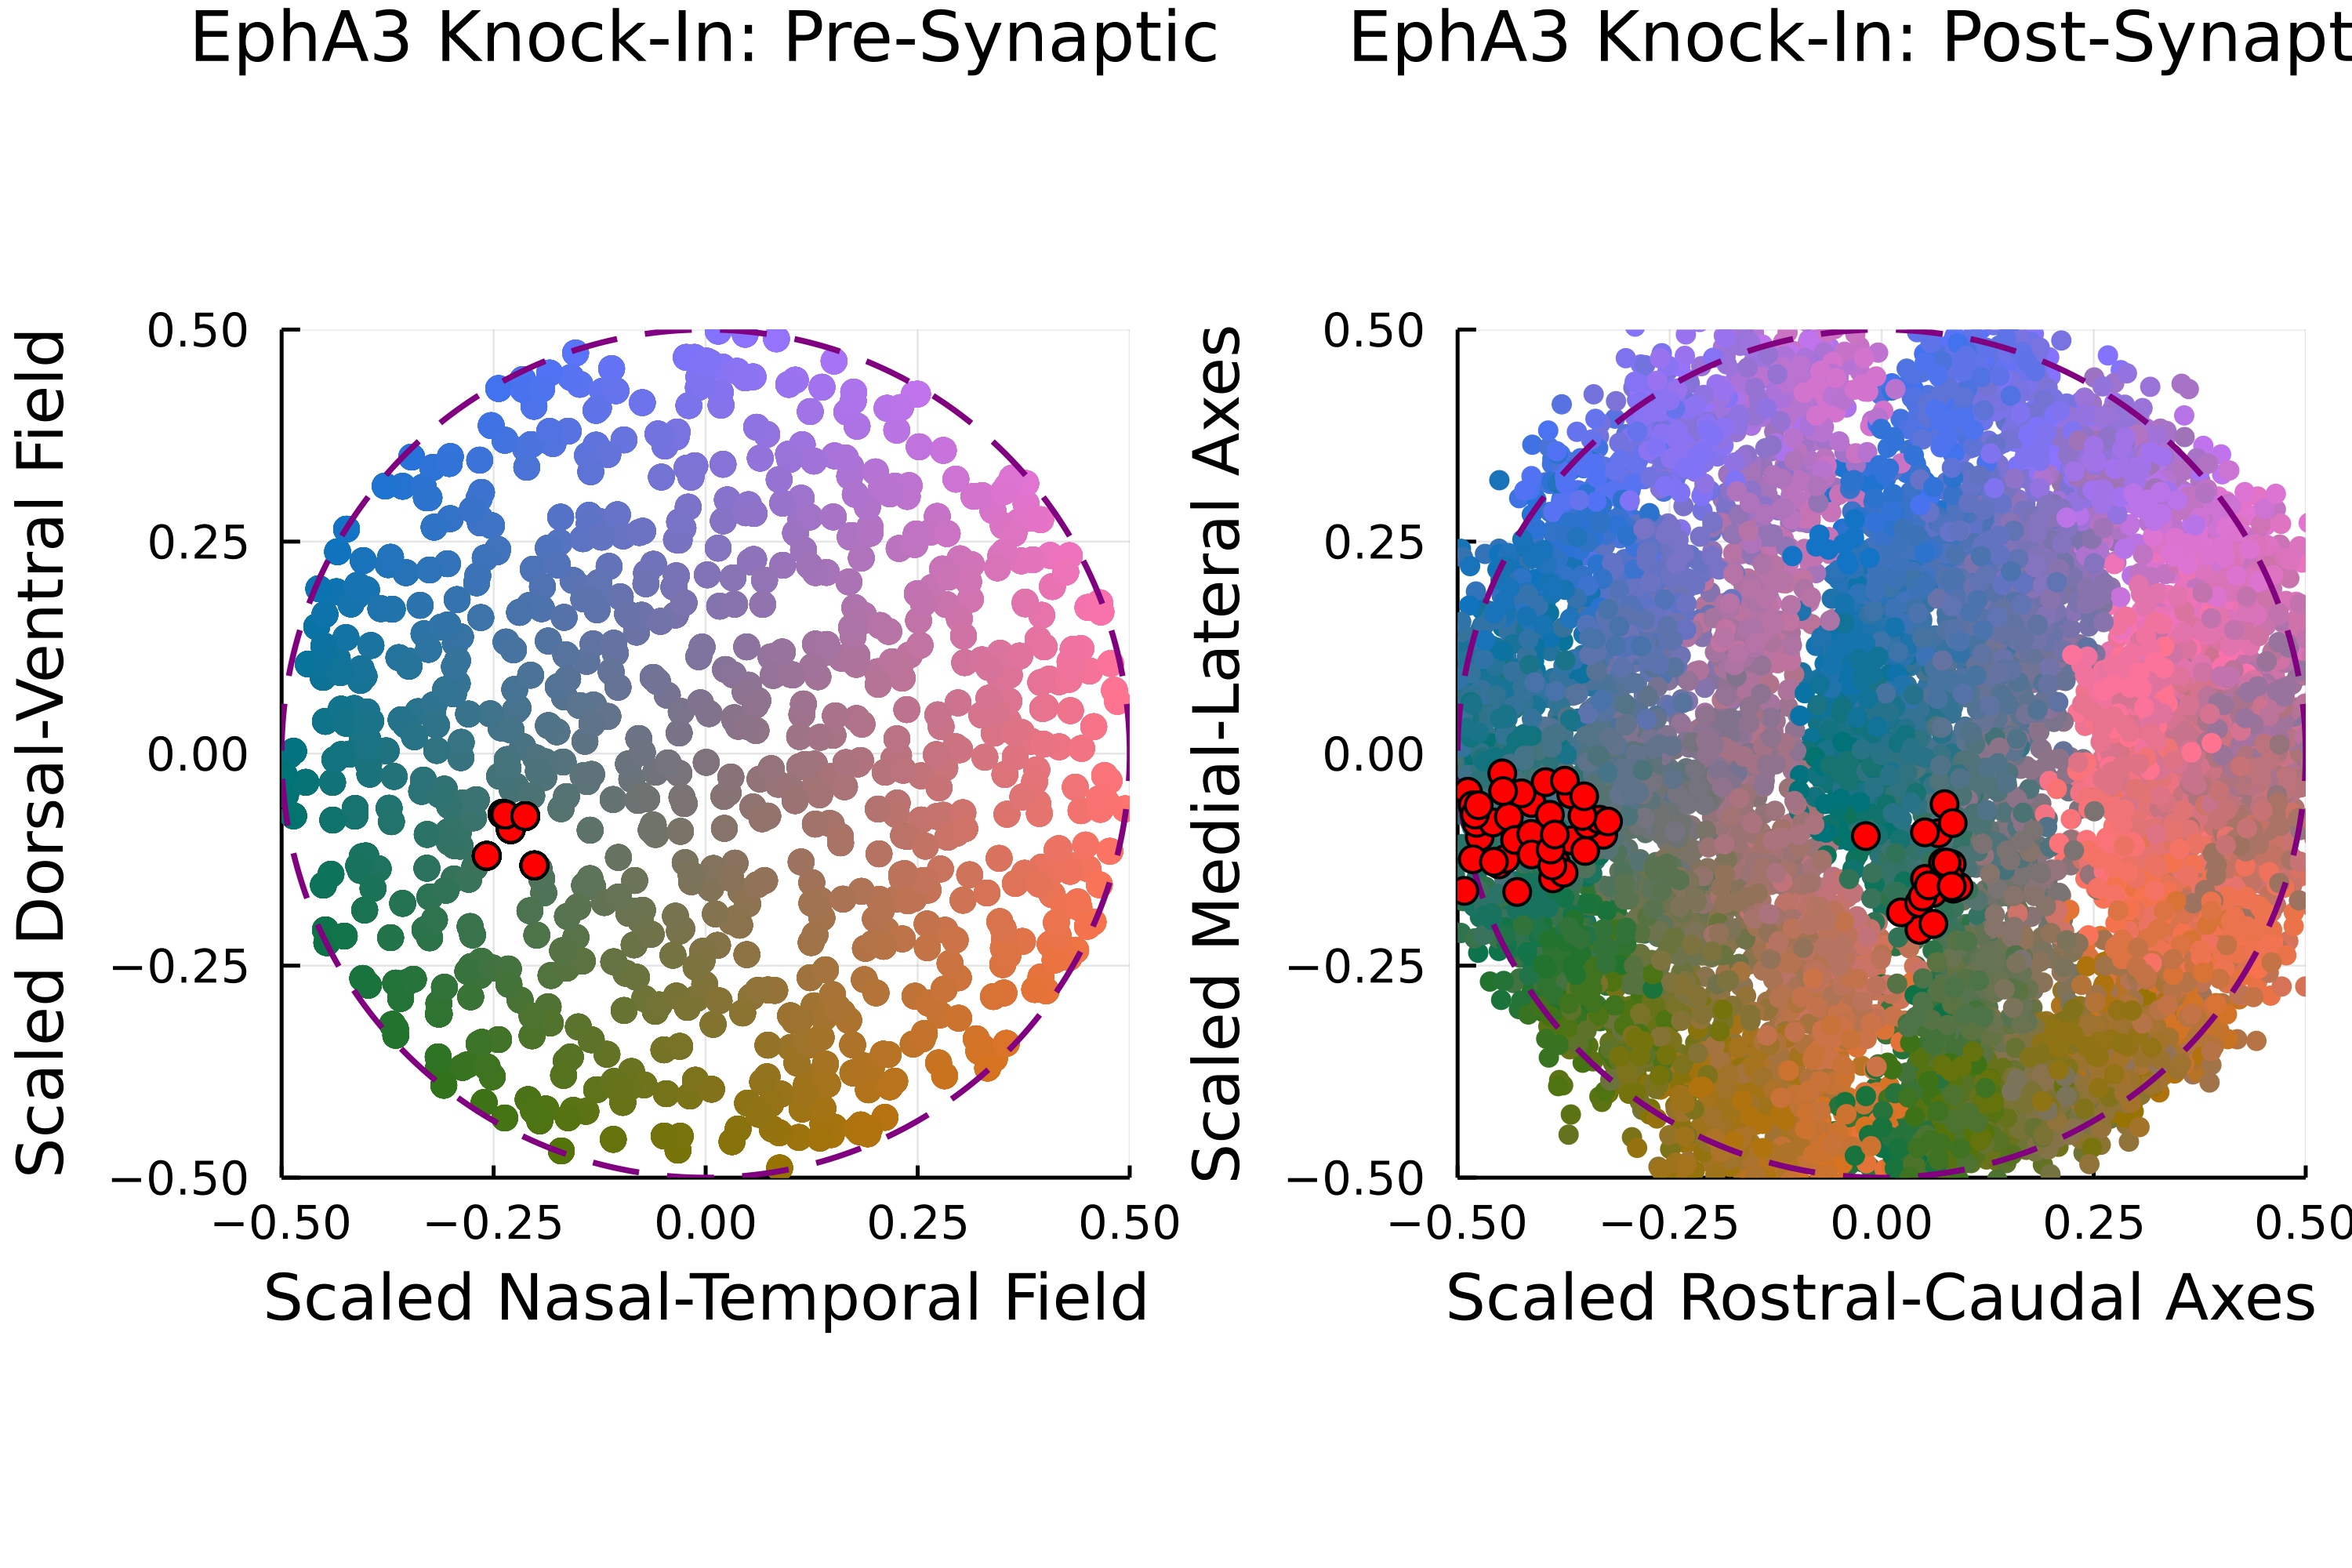
\includegraphics[width=\textwidth]{images/distributed_kernels/figure_distributed_kernels_EphA3}
		\caption{}
	\end{subfigure}
	~
	\begin{subfigure}{0.5\textwidth}
		\centering
		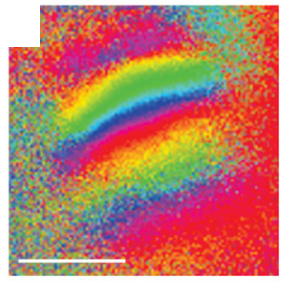
\includegraphics[width=\textwidth]{images/distributed_kernels/ephA3hom}
		\caption{}
	\end{subfigure}
	\qquad\qquad
	\begin{subfigure}{0.3\textwidth}
		\centering
		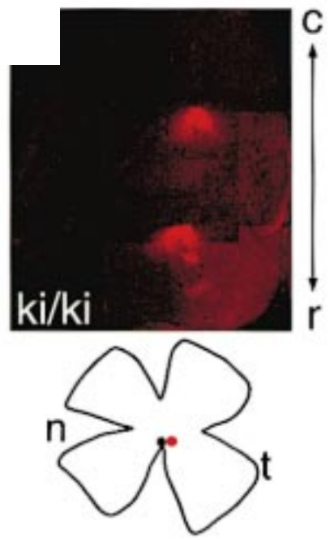
\includegraphics[width=\textwidth]{images/distributed_kernels/epha3anatomical}
		\caption{}
	\end{subfigure}
	\def\c{A rainbow plot for the EphA3 phenotype.}
	\caption[\c]{\label{fig:epha3_rainbow} A rainbow plot for the EphA3 phenotype is shown in (a). There is a normal topographic projection along the lateral-medial axes and a bifurcation in the rostral-caudal axis. The bifurcation happens at approximately the midpoint of the target region and results in a duplication of the pre-synaptic field in both rostral and caudal regions. An optical imaging scan of the azimuthal axis reveals this duplicated map in panel (b); figure adapted from Owens et. al. (2015) \cite{Owens2015-zv}. A retinal injection is shown in red and is comparable to analogous anatomical injections which are shown in (c); figure adapted from Brown et. al. (2000) \cite{Brown2000-da}. }
\end{figure}


\begin{figure}[hbt!]
	\centering
	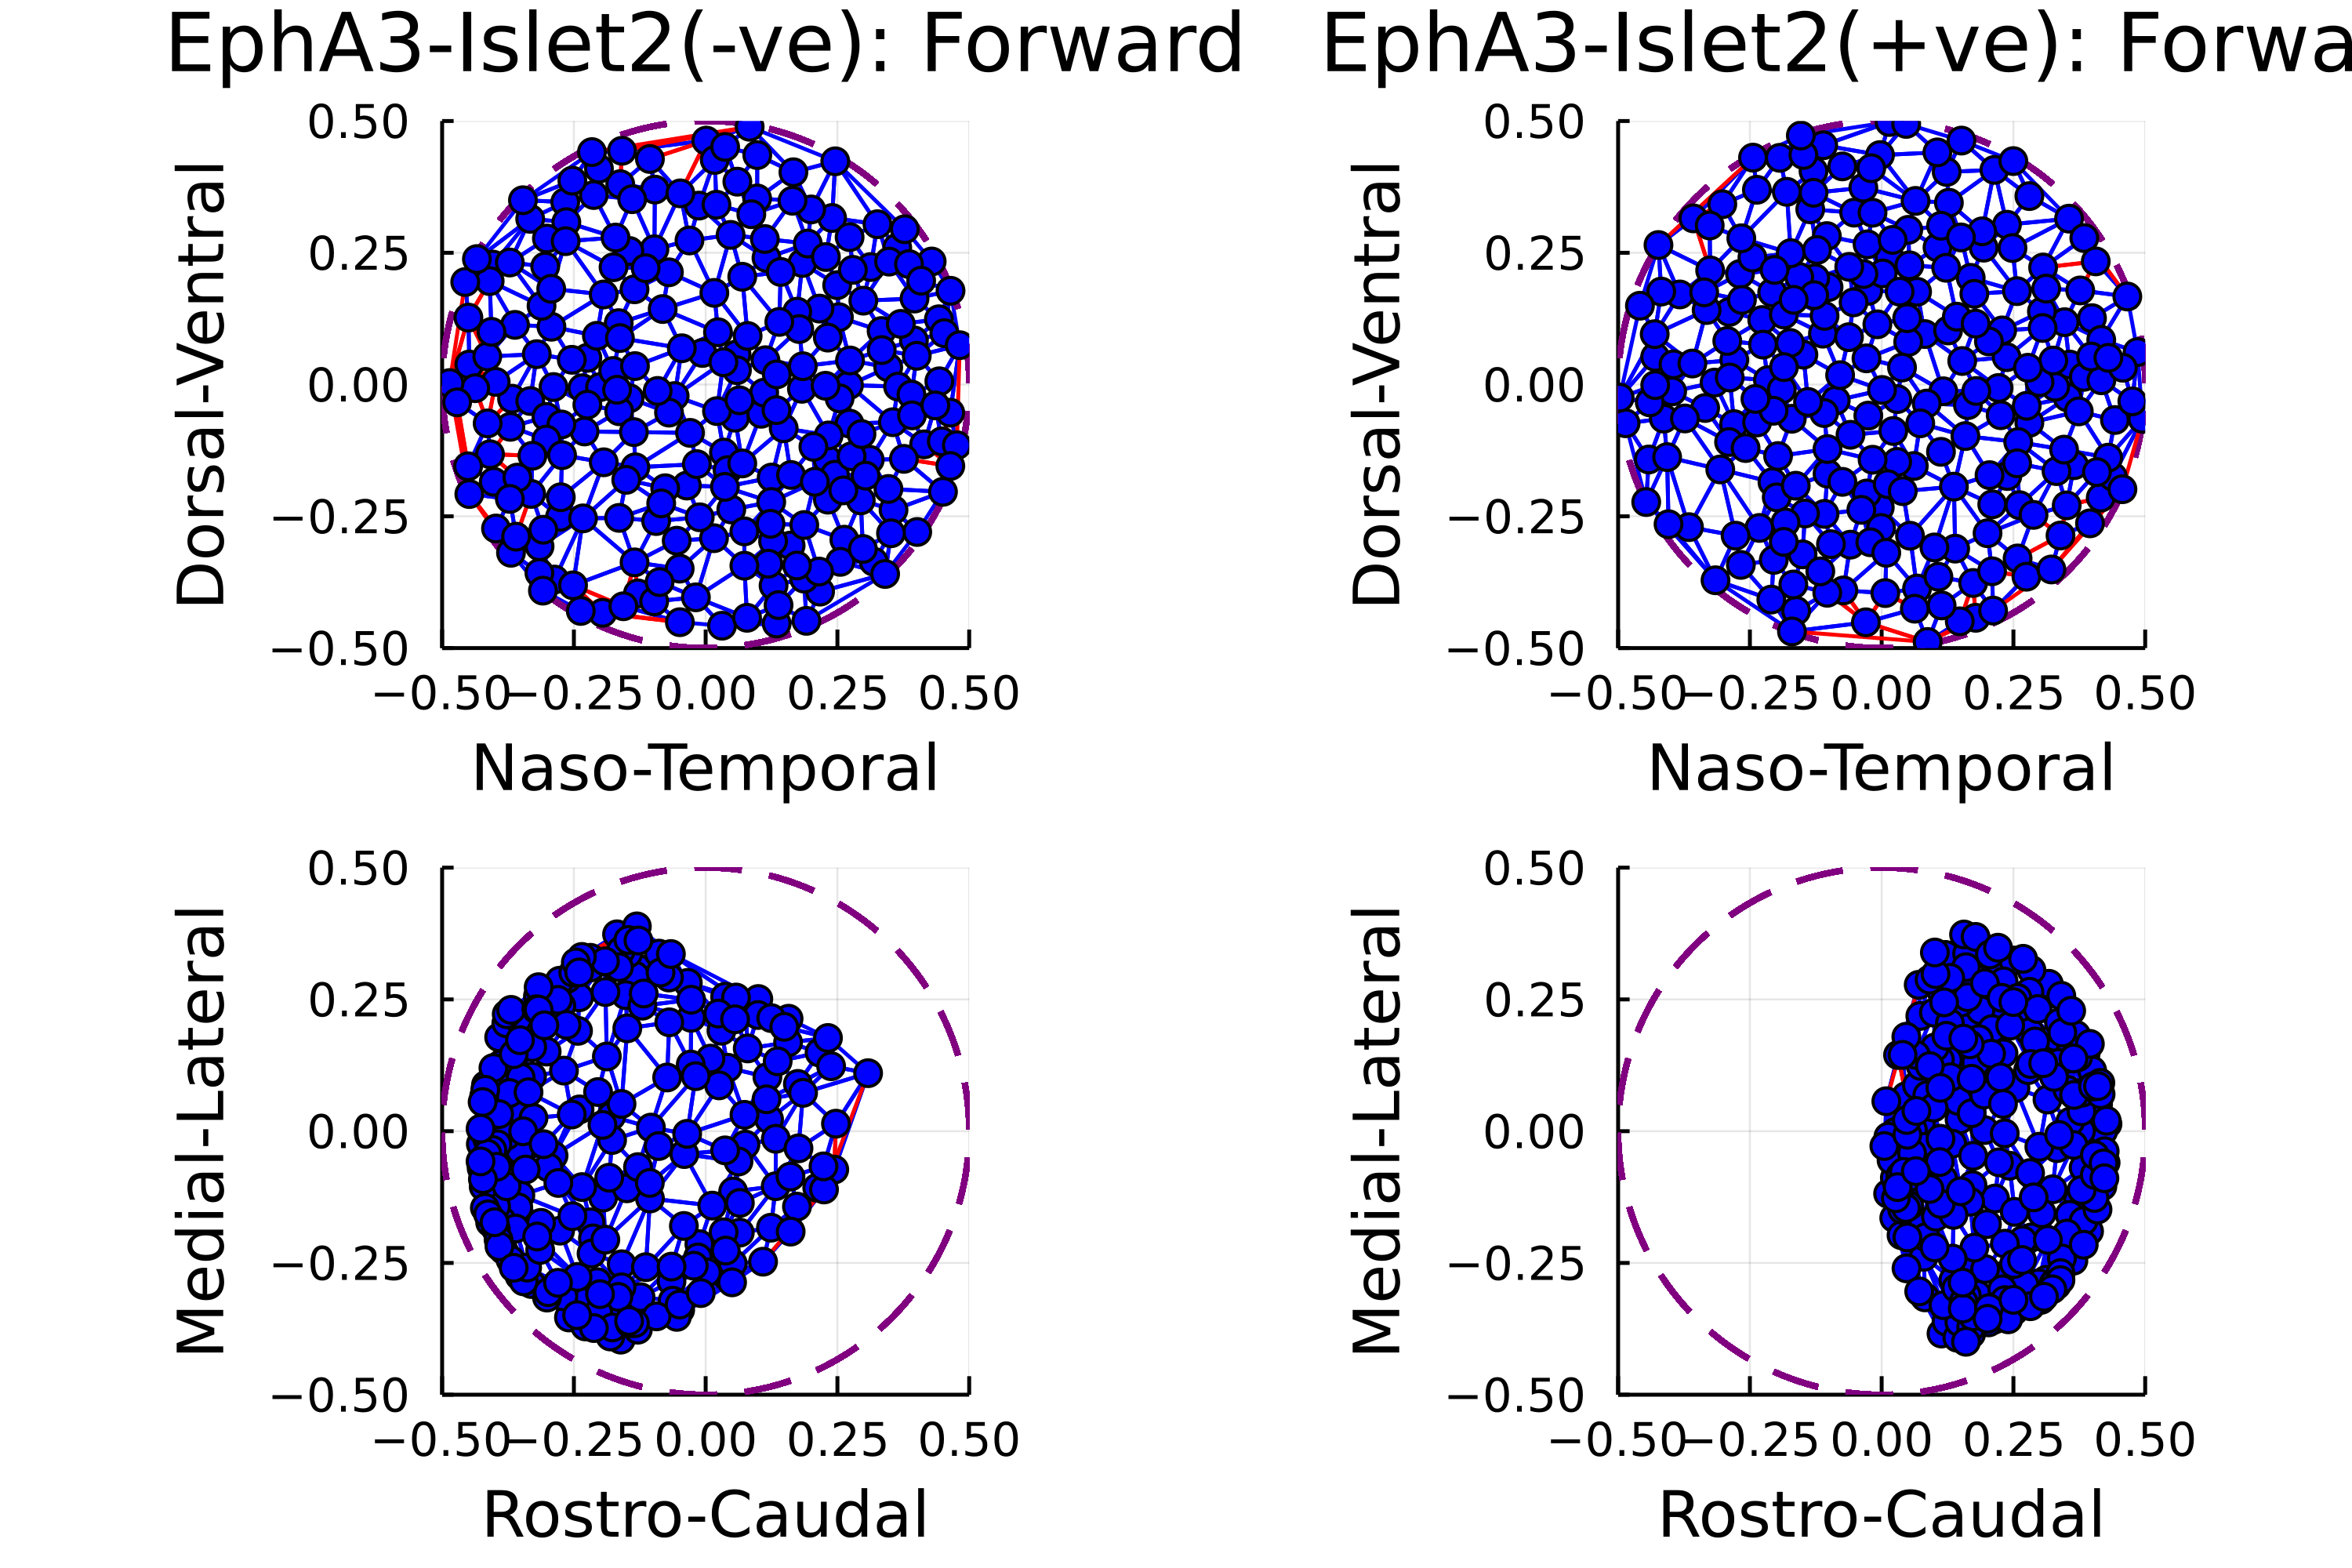
\includegraphics[width=\textwidth]{images/distributed_kernels/figure_lattice_EphA3_pre}

	\def\c{Forward lattice plots for the homozygous EphA3 knock-in phenotype showing the projection from wild-type cells and the projection of cells containing additional EphA3.}
	\caption[\c]{\label{fig:epha3_lattice_pre} Forward lattice plots for the EphA3 phenotype with (a) showing the projection from wild-type cells and (b) showing the projection of cells containing additional EphA3. The wild-type cells cover the colliculus area while the EphA3 tagged cells are restricted to the caudal region. This is consistent with the modelling performed in Chapter \ref{chapter:lattice}.}
\end{figure}

\begin{figure}[hbt!]
	\centering
	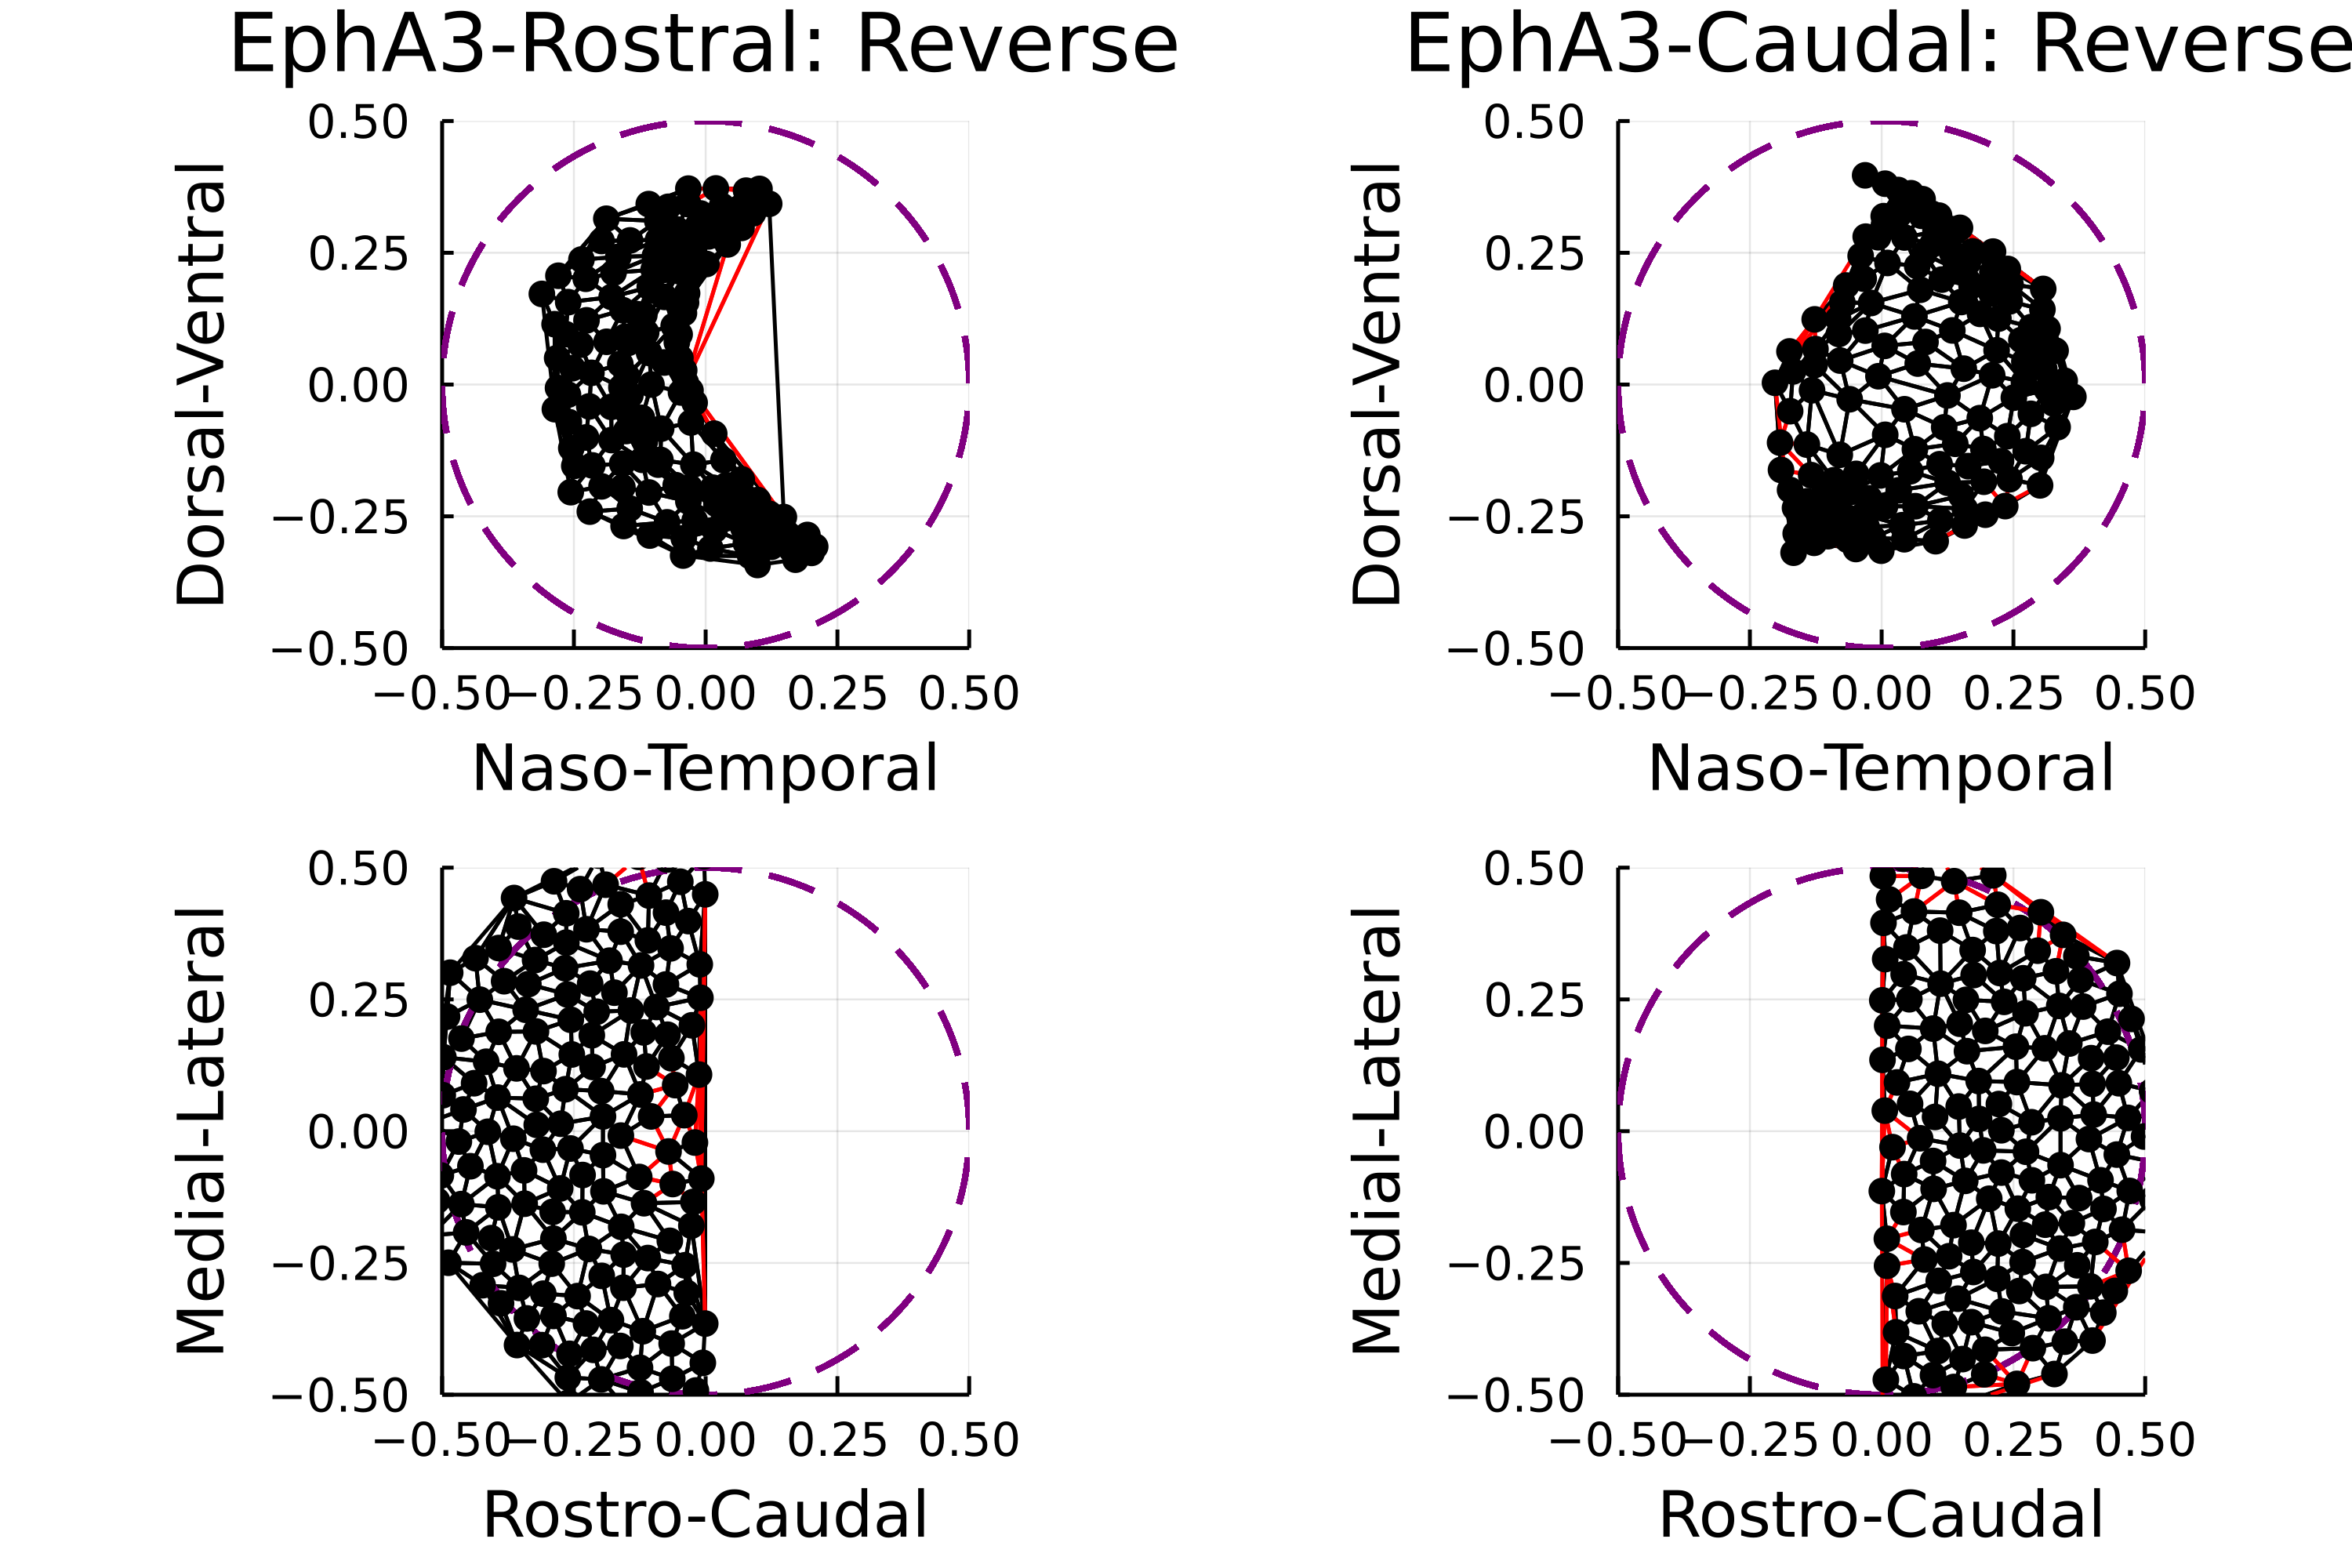
\includegraphics[width=\textwidth]{images/distributed_kernels/figure_lattice_EphA3_post}
	\def\c{Reverse lattice plots for the homozygous EphA3 knock-in phenotype which show the rostral and caudal maps.}
	\caption[\c]{\label{fig:epha3_lattice_post} Reverse lattice plots for the EphA3 phenotype which show the rostral (a) and caudal (b) maps. Both of these maps cover a significant portion of the visual field and have overlap with each other. This is consistent with both the modelling performed in in Chapter \ref{chapter:lattice} and the analysis of the mutant data. The mutant data was constructed on the azimuthal-elevational scans which correspond quite well, but not precisely, to the nasal-temporal and dorsal-ventral components of the visual field. This aberration will slightly modify reconstructed maps and should be examined further.}
\end{figure}
\newpage
\subsection{$\beta2$ knock-out}
The $\beta2$ knock-out has the effect of changing the spatio-temporal properties of the spontaneous activity patterns generated in the retina before eye opening \cite{Burbridge2014-ib, Xu2011-mt, Dhande2011-gj, Stafford2009}. The effect of this is to reduce the precision with which the final map is formed; retinal afferents have enlarged arbors \cite{McLaughlin2003-co, Burbridge2014-ib, Xu2011-mt}. The mechanism by which this process acts is assumed to be Hebbian on the aggregate correlation of the activity patterns which follow an exponentially decaying relationship in distance. A framework in which this hypothesis can be rigorously analysed was developed in Chapter \ref{chapter:neuralstdp} and under some symmetry assumptions this assumption can be shown to be sound. This knock-out is simulated by increasing the correlation width to $d_r=0.25$ and scaling down the correlation strength $\gamma = 10^{-3}$. The rainbow plot presented in Figure \ref{fig:beta2rainbow} shows that topographic ordering is largely preserved but the retinal injection highlighted in red shows an enlarging of the anatomical arbor. This is consistent with retinal injections performed on $\beta2$ mice \cite{Burbridge2014-ib, McLaughlin2003-yy}. The lattice plots presented in Figure \ref{fig:beta2lattice} show a relatively ordered projection with mapping errors occurring in a ring around the boundary. While no data derived lattice plots exist for the $\beta2$ knock-out a lattice analysis of a combined EphrinA2A3A5 triple knock-out and $\beta2$ knock-out reveal that the activity disruptions remove the residual order found at the boundaries of the map and this model is consistent with that result \cite{Willshaw2014-ms}.
\begin{figure}
	\begin{subfigure}{\textwidth}
		\centering
		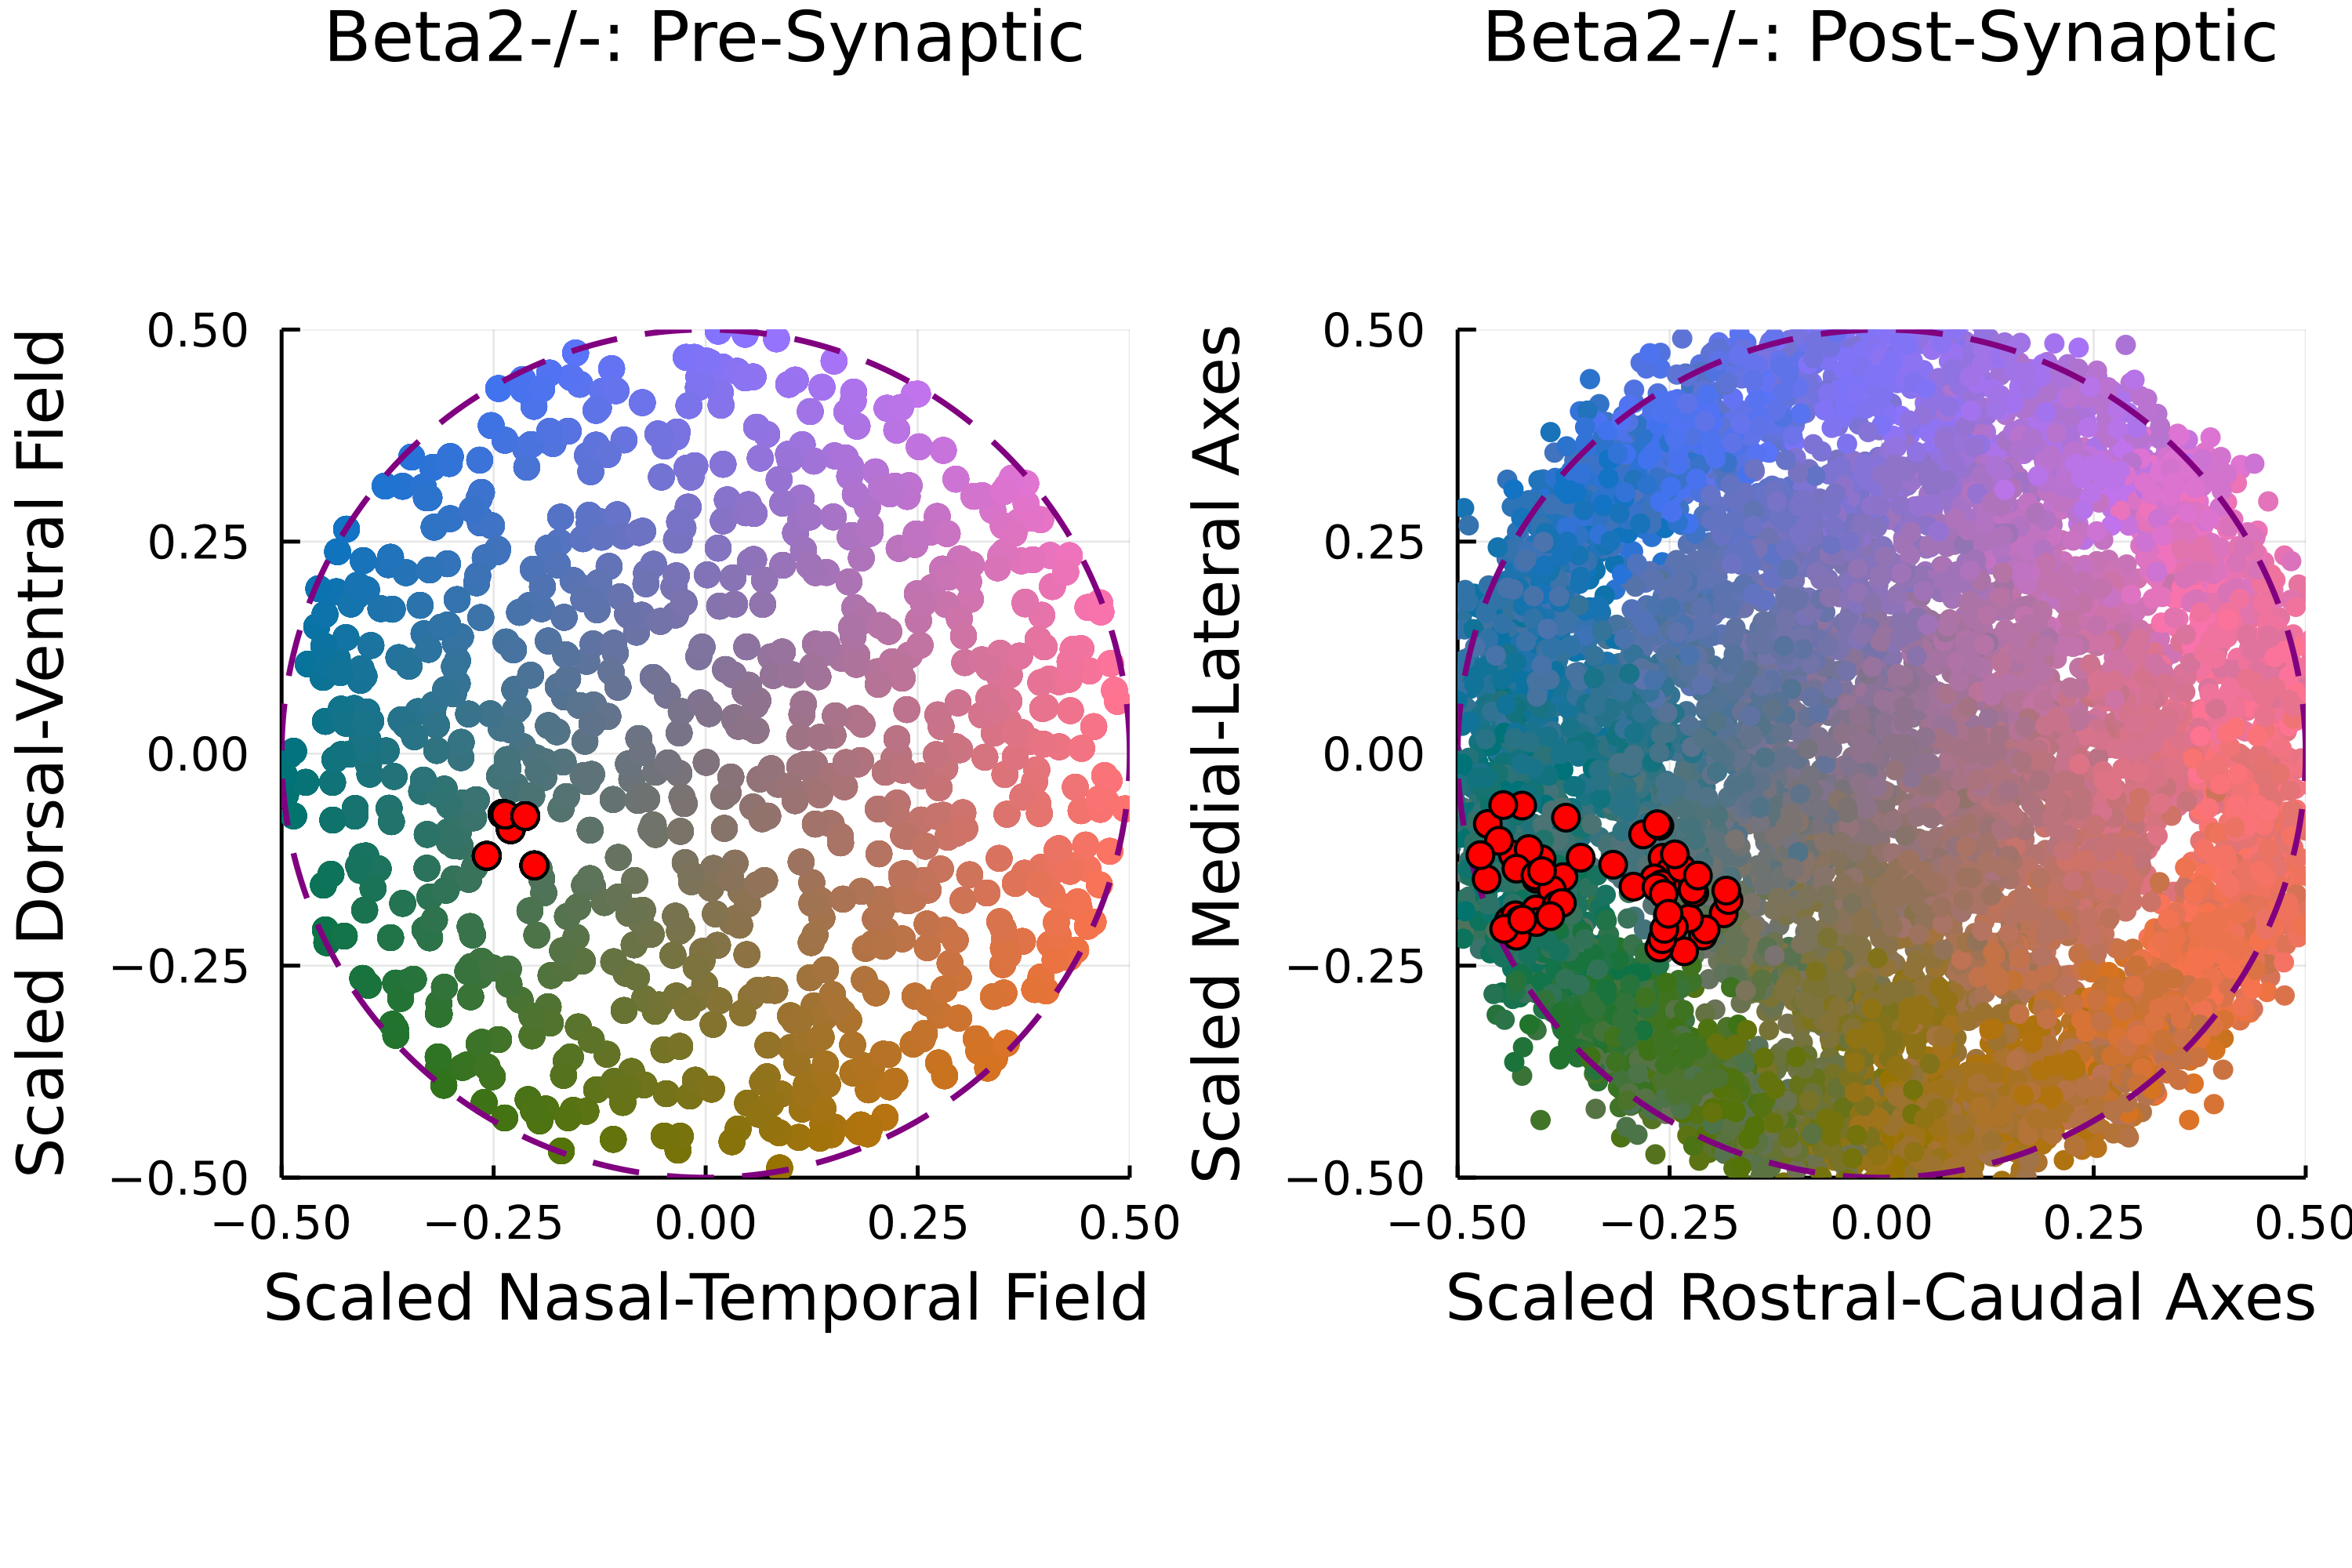
\includegraphics[width=\textwidth]{images/distributed_kernels/figure_distributed_kernels_Beta2}
		\caption{}
	\end{subfigure}
	~
	\begin{subfigure}{\textwidth}
		\centering
		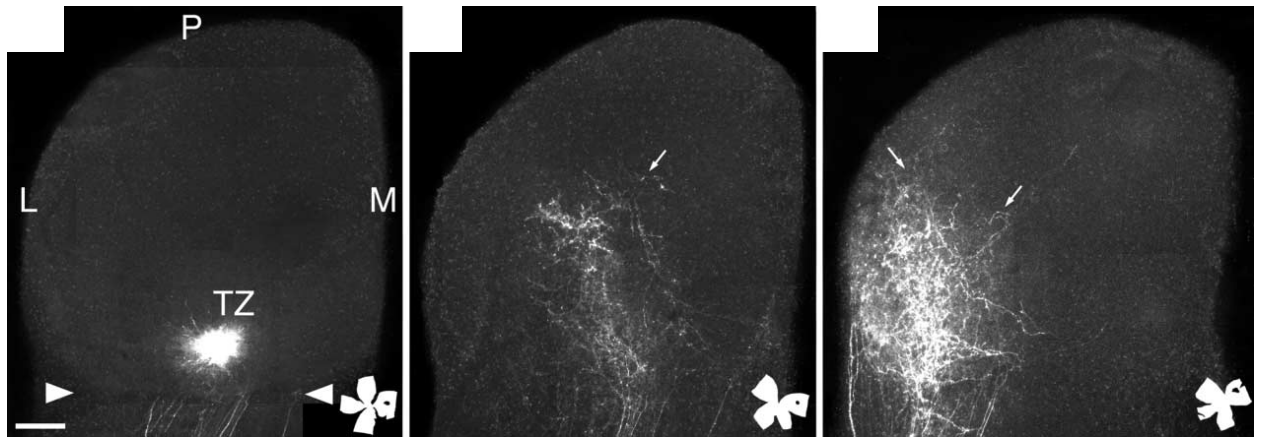
\includegraphics[width=\textwidth]{images/distributed_kernels/beta2}
		\caption{}
	\end{subfigure}
	\def\c{A rainbow plot of the $\beta2$ knock-out is presented.}
	\caption[\c]{\label{fig:beta2rainbow} A rainbow plot of the $\beta2$ knock-out is presented in (a) showing that the topographic order is largely maintained. The retinal injection shown in red shows an enlarged projection zone compared to wild-type (Figure \ref{fig:wtrainbow}) and this is comparable to retinal injections performed at P8 shown in the two rightmost panels of with the left showing a wild-type (b); figure adapted from McLaughlin et. al. (2003) \cite{McLaughlin2003-yy}.}
\end{figure}
\begin{figure}
	\begin{subfigure}{0.6\textwidth}
		\centering
		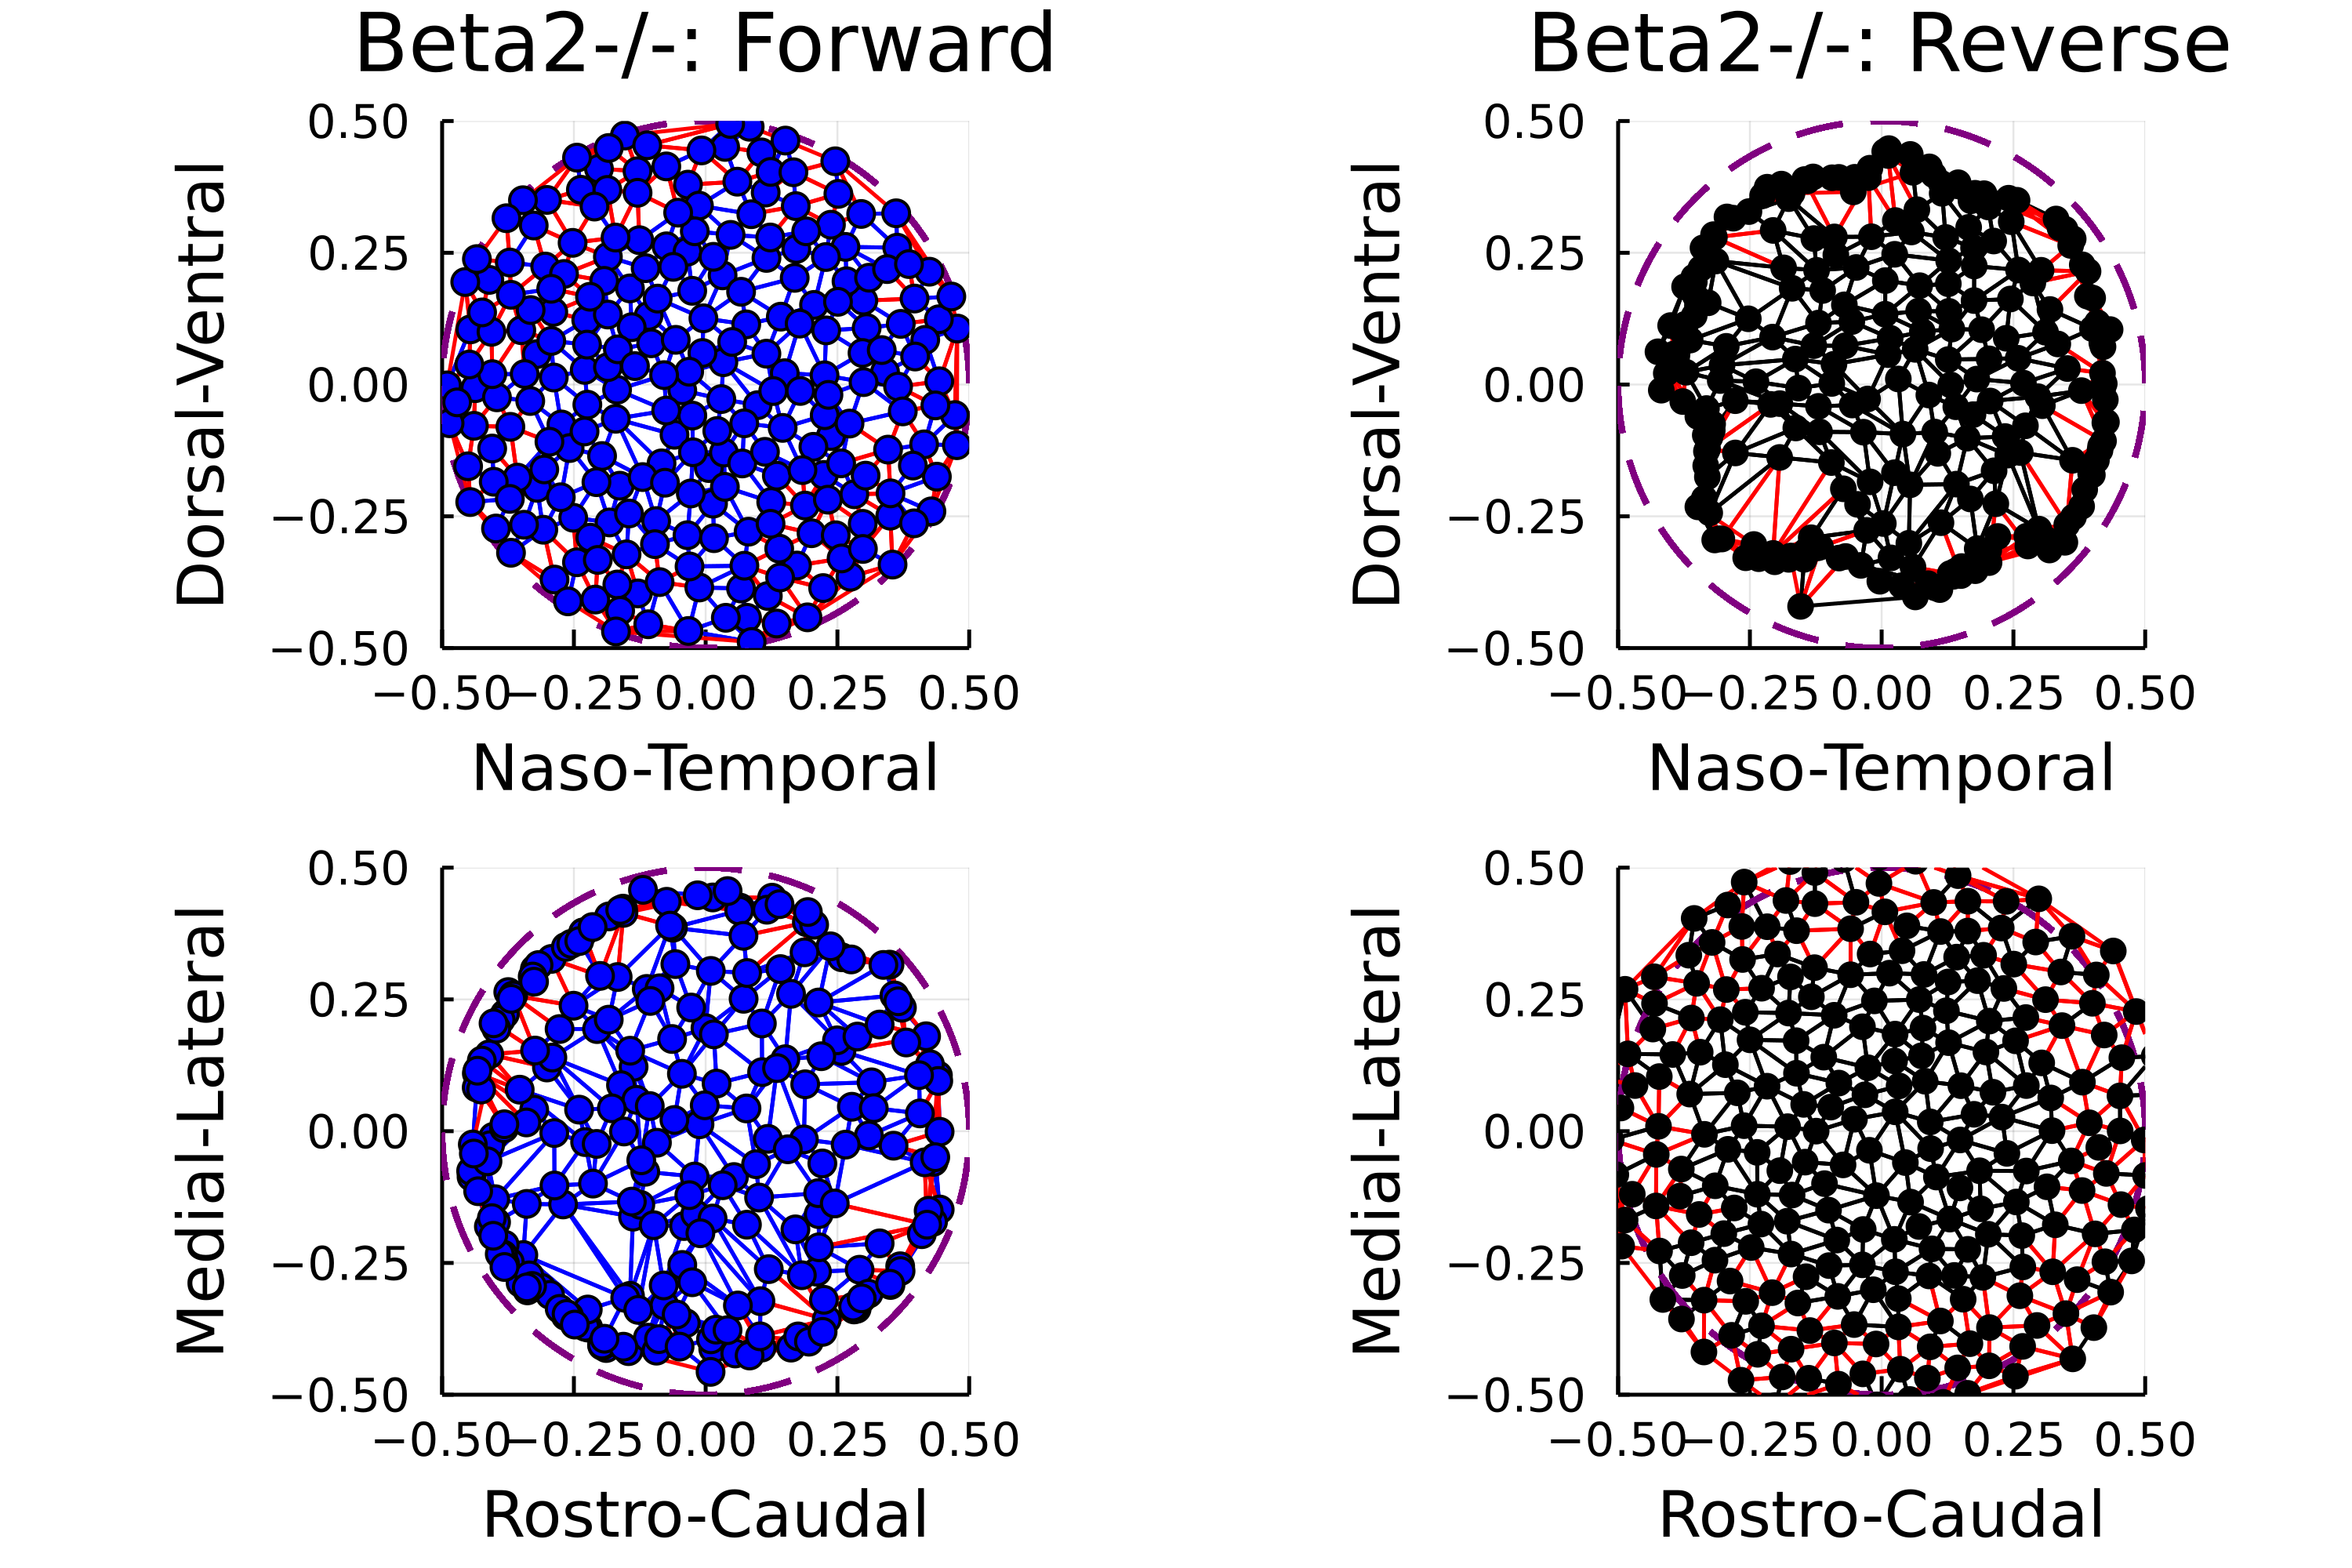
\includegraphics[width=\textwidth]{images/distributed_kernels/figure_lattice_Beta2}	
		\caption{}
	\end{subfigure}
	\begin{subfigure}{0.4\textwidth}
		\centering
		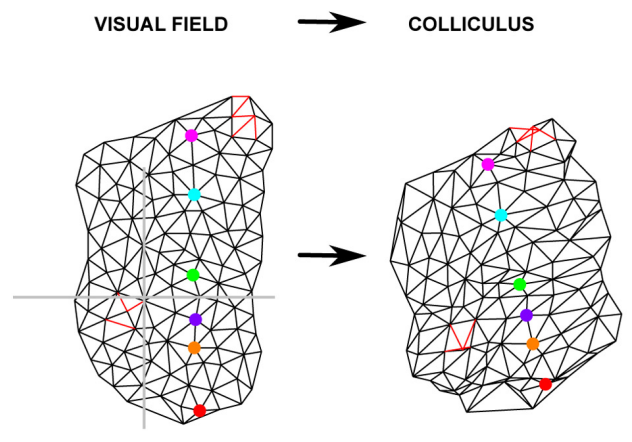
\includegraphics[width=\textwidth]{images/distributed_kernels/latticeB2}	
		\caption{}
	\end{subfigure}
	\def\c{Forward and reverse lattice plots for $\beta2^{-/-}$ mutant are shown.}
	\caption[\c]{\label{fig:beta2lattice} Forward and reverse lattice plots for $\beta2^{-/-}$ mutant are shown in panel (a). The structure of the maps is relatively well ordered in both directions with small defects occurring on the boundaries. This is consistent with the lattice method analysis applied to real data in the forward direction and shown in panel (b); figure adapted from Willshaw et. al. (2014) \cite{Willshaw2014-ms}.}
\end{figure}

The $\beta2$ development is notably slower than that of wild-type mice as demonstrated in the analysis presented by Lyngholm et. al. (2019) \cite{Lyngholm2019-fs}. To analyse the development in the model an injection covering 5\% of the retina is made at the retinal position (0.1, 0.1) and a measure of projective field is estimated as the maximal ellipsoid that covers the points in the projective field. The ellipsoid is constructed by taking the half the range of the projective points in each dimension as the ellipse axes $r_1$ and $r_2$. The ellipse area is calculated as $\pi r_1 r_2$. The results of the time evolution of this projective field area are shown in Figure \ref{fig:beta2WTprojectionevolution}. The projective field area is initially small as the retinal contacts are located in a restricted portion of the colliculus, grows through the chemotactic development stage, and then experiences non-linear retraction followed by growth, and then finally relaxes into a steady state. The wild-type and $\beta2^{-/-}$ mutant both follow this pattern but notably the wild-type establishes this steady state sooner than the $\beta2^{-/-}$ mutant. 

\begin{figure}[hbt!]
	\centering
	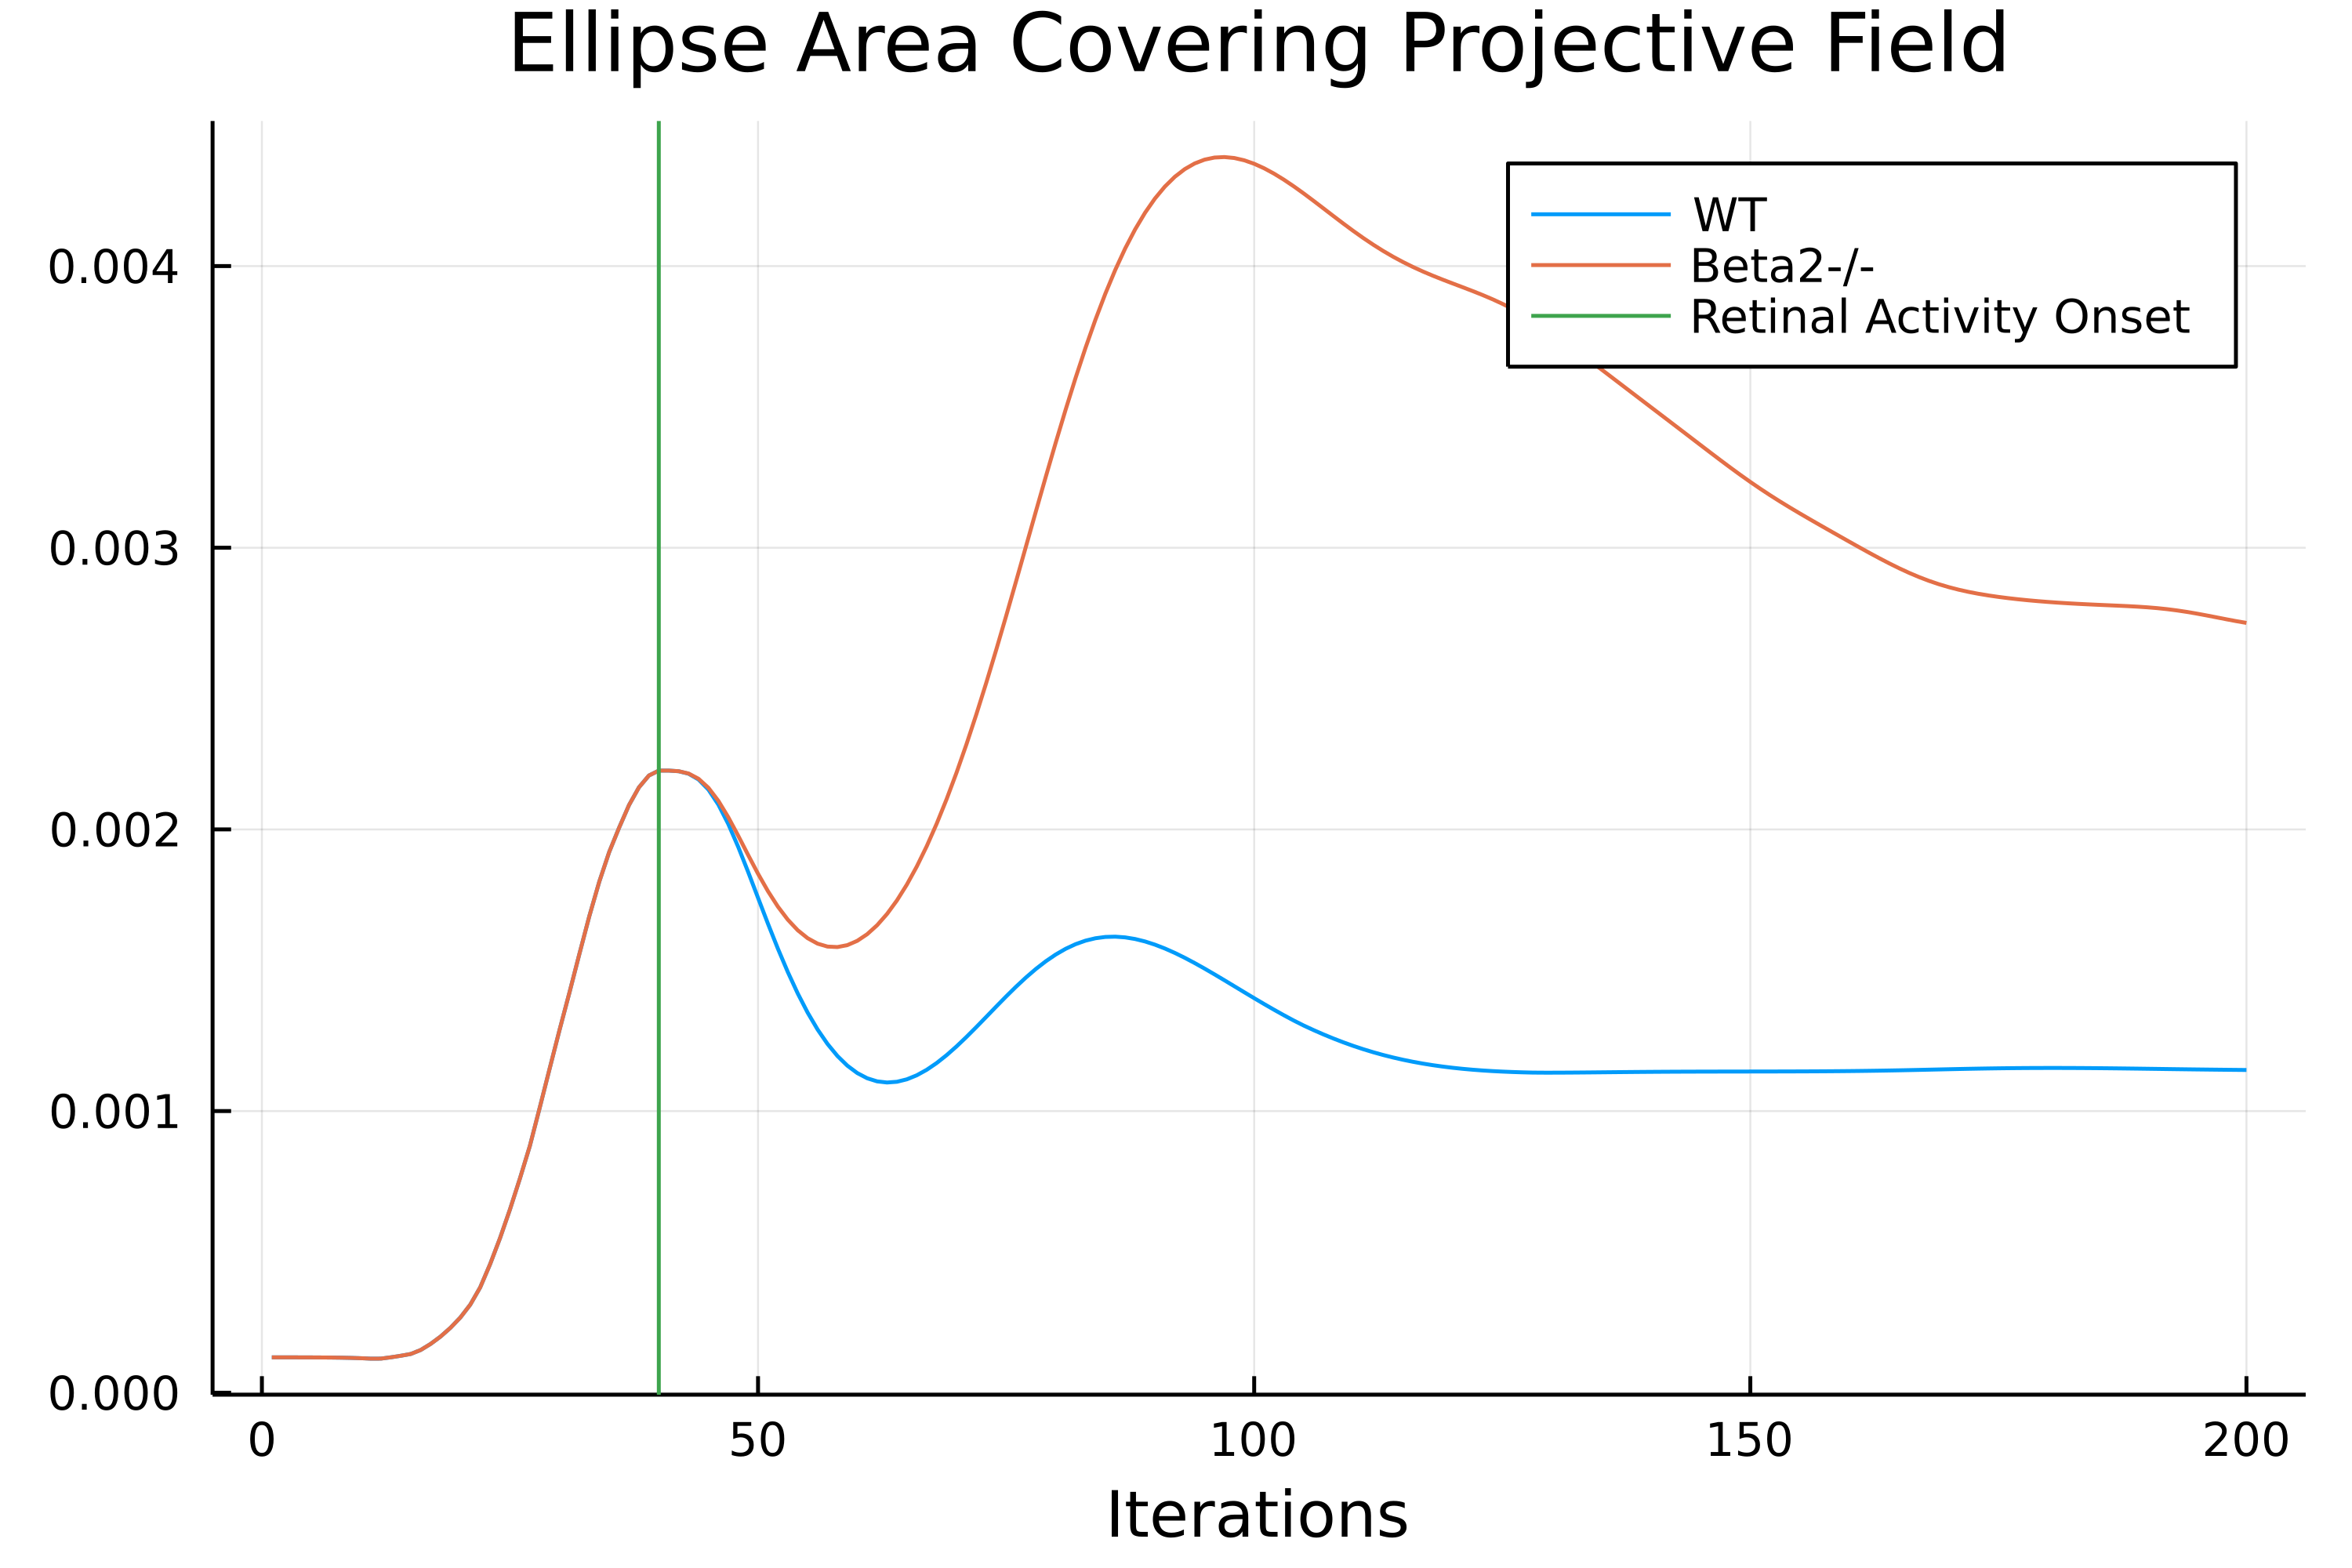
\includegraphics[width=\textwidth]{images/distributed_kernels/figure_beta2vsWTprojection}
	\def\c{Time course evolution of the area of an ellipsoid covering the projective field of a retinal injection made at retinal location (0.1, 0.1). }
	\caption[\c]{\label{fig:beta2WTprojectionevolution} \c The ellipse axes are found by taking half the range of points along each dimension which a 5\% area of the retina centred at the retinal location project project to. The area is found using the ellipse area formula. The projection area for the $\beta2^{-/-}$ knock-out is refined at a slower rate than that of wild-type which is in accordance with data \cite{Lyngholm2019-fs}.}
\end{figure}
\newpage
\section{Discussion}
A modelling framework was developed by integrating the salient and necessary features of existing unified models which have been shown to provide good explanations of existing data but are too computationally demanding to perform the necessary parameter robustness and statistical analyses to validate them; see Chapter \ref{sec:models}. The model is an energy based formulation and is flexibly designed to be linear combinations mechanisms which allows the inclusion of additional mechanisms should new experimental evidence reveal that they are required. To assess the model the methodology illustrated by Hjorth et. al. (2015) was followed choosing the calibration phenotype to be wild-type \cite{Hjorth2015-le}. To demonstrate that the model was at least as parsimonious as the existing frameworks it validated against the phenotypes in the pipeline as well as examining an additional mutant: the $\beta2$ knock-out. These phenotypes were reproduced faithfully in line with experimental data and corroborating the new observations made about the EphA3 phenotype using the Tsigankov-Koulakov model in the Chapter \ref{chapter:lattice}. 
\paragraph{$Math5$ knock-out}
The $Math5^{-/-}$ phenotype has been particularly challenging for retinotopic models with the most successful being the Tsigankov-Koulakov and generalised Gierer models \cite{Triplett2011-jk, Sterratt2013-ev}. The reason these are successful is because they are Type I graded matching models and do not prescribe retinotopically correct termination zones on the basis of gradients but rather allow for relative sorting with gradient biases and a competitive mechanism. The competitive mechanism in the generalised Gierer model is relatively easy to interpret amounting to a multiplicative normalisation while the mechanism in the Tsigankov-Koulakov model is difficult and adds significant parameter complexity --- another 6 dimensions. The competition mechanism in the Distributed Kernels model provides similar benefits with a natural interpretation: afferents diffuse away from areas which have large concentrations and into regions of low concentration. The prediction that the model makes is that even though the $Math5^{-/-}$ projection is restricted to a quadrant of the colliculus the ordering of the map is highly topographic. There has been no measurements of topographic order in the $Math5^{-/-}$ mutant and this is a direction of future research.
\paragraph{$\beta2$ knock-out}
The $\beta2^{-/-}$ phenotype has been established as the default experimental system with which to understand developmental activity patterns in the visual system \cite{Seabrook2017-fa, Burbridge2014-ib, Zhang2017-hs, Xu2015-uc}. Despite this there have been relatively few quantitative modelling studies which aim to understand its effects and of these very few are quantitative \cite{Lyngholm2019-fs, Tikidji-Hamburyan2016-sn, Godfrey2009-ts}. The work in Chapter \ref{chapter:neuralstdp} provided a framework with which to understand both the spatial-temporal structure of the waves and resulting effects on the development of topography, and the statistical methodology by which to understand its parameter space more generally. It also provided a reduction of the effect to just spatial correlations in the limiting case of equiproportionally distributed waves. Therefore, it is encouraging that in this limiting case this 2D model can reproduce the effect of the knock-out. 

However, there is a body of evidence that shows that the waves are not equiproportionally distributed in the retina --- they show directional biases \cite{Ackman2012-uu, Ackman2014-tj}. There is also a growing body of evidence that feature maps such as orientation selectivity are present in sub-cortical structures such as the superior colliculus \cite{Ahmadlou2015-jw, Feinberg2015-eu}. This raises a significant challenge for the model as it cannot represent spatial asymmetry with a spatially symmetric correlation function and these correlations must therefore be decomposed into a less efficient correlation matrix. It would be more appropriate to examine these questions with natural 2D extension of the model proposed in Chapter \ref{chapter:neuralstdp}. It also calls into a question a theoretical result of the Elastic Net model discussed in \ref{sec:heuristics} whereby the model predicts a distortion of retinotopy near regions of rapid change in orientation selectivity. The superior colliculus does not demonstrate topographic distortions along the lines of orientation preference under lattice analysis. There are two possibilities: one it is an averaging effect of the measuring and/or analysis process and the distortion happens below some measurable threshold, two the Elastic Net model can be revisited and updated to predict this fact.
\paragraph{Developmental Time}
As discussed in Section \ref{model:time} existing models of retinotopic development do not account for time in a principled manner. The Tsigankov-Koulakov model was recently applied to a dataset which outlined the developmental time course of the $\beta2^{-/-}$ mutant and wild-type mouse \cite{Lyngholm2019-fs}. The model was not able to capture the critical developmental delays observed in the $\beta2^{-/-}$ mutant mouse and this is most likely because the minimisation procedure used is a stochastic sampler which asymptotically converges to a steady-state distribution but does not evolve to this distribution in a temporally interpretable fashion. The model presented here can capture the phenomenon of developmental delay and large termination zones observed in the $\beta^{-/-}$ mutant using a simple tracer injection methodology \cite{Lyngholm2019-fs, McLaughlin2003-yy}. Notably, this did not require parameter tuning of mechanisms other than neural activity. The notion of time remains to be precisely quantified because the gradient descent optimiser used involves adaptive momentum and this is difficult to formally map onto developmental processes. Calibrating the model iterations to time is an immediate line of future research. 
\paragraph{Computational Efficiency}
The Distributed Kernels Model is computationally efficient and this is the principal result of this work: the work in Chapter \ref{chapter:lattice} showed that significant comprises needed to be made in order to perform statistical analysis with the Tsigankov-Koulakov model. It was necessary that any proposed new model make sufficiently similar predictions to the Tsigankov-Koulakov model which offers adequate explanations for available data. It is also not surprising that it makes similar predictions because it was composed of the abstract features that drive the model; albeit with fewer parameters. However, the Tsigankov-Koulakov model is computationally demanding and unintuitive this limits the generality of conclusions made from it. The work in Chapter \ref{chapter:lattice} showed the both the hazards of reasoning from the model minimisation procedures with Owens et. al. (2015) proposing a stochastic interaction between activity and chemotaxis mechanisms, as well as the infeasibility of doing the large scale parameter and statistical studies necessary to reason about it robustly. 

The model proposed here improves the computational efficiency while retaining predictability in two ways: using adaptive rate gradient descent based operators to find local minima effectively, and parallelising all computations to run on GPU architectures. The minimisation scheme is different to the Metropolis-Hastings type scheme employed in the Tsigankov-Koulakov model and converges to a single map, rather than a distribution of possible maps. This is a desirable feature in model assessment because generation of representative samples of potential model output is not required. The scheme converges in a reasonable small number of iterations and alongside the parallelisation results in 100 times speed-up over the Tsigankov-Koulakov model. The algorithm scales sub-linearly as opposed to $O(n^3)$ and so this performance gap should increase for an increasing number of cells. This significant boost in performance is notable as no optimisation was performed on the code --- the back-propagation is naively computed using a memory hungry auxiliary package and the calculations are performed with Julia's inbuilt lazy broadcast and linear algebra. There are a number of potential optimisations that can be made to enhance performance further. These considerations mean that this model is a good candidate for performing the Bayesian parameter analysis combining all data-sets and robustness studies which are currently needed; see Section \ref{model:assessment}. It also is easily falsifiable against new experimental data which is a desirable feature of a model.
\paragraph{Limitations}
The studies presented here have several key limitations: they are phenomenological and the parameters have been hand-tuned. A number of different mutant genotypes were examined and the model was shown to be able to reproduce their phenotypes with a selection of specific parameters. These were modified only in the mechanisms which the genotypic mutation is likely to affect but they were not chosen in a rigorous fashion, rather following in the convention of other retinotopic models. A desirable feature of the model is that it is able to capture the developmental delays of the $\beta2^{-/-}$ mutant without extensive parameter tuning which has been a failing of existing models \cite{Lyngholm2019-fs}. However, this was a phenomenological description rather than a quantitatively predictive one and thus needs further calibration. The motivation for developing the model was largely to have a framework in which parameters can be derived from data rigorously and allow the model to make quantitative predictions and therefore this is a principal vector of future research.
\paragraph{Future Work}
The most immediate line of future research is extensive interrogation of biological data to develop a theoretical understanding of the model parameter space and the implications this has for understanding how developmental mechanisms interact with each other. The methodology developed in Chapter \ref{chapter:lattice} whereby optical imaging scans are generated using an underlying anatomical model and summarised by statistics of the lattice method is the most straightforward way to proceed with this. The biggest challenge here is the availability of data. The dataset from Owens et. al. (2015) is only partially available and there is no existing centralised repository of data to draw from: developing such a repository would be invaluable to both validating this model but also any other model or data analysis technique and be developed following existing repository examples \cite{Owens2015-zv, Eglen2014-fo}. 

The model could be further applied to answer key features about the developmental time course of various mutants. A necessary first step would be calibrating the model to known developmental time points and this could be achieved by a pipeline which follows the data analysis procedure presented by Lyngholm et. al. (2019) \cite{Lyngholm2019-fs}. After calibration the model could then be interrogated to make time-sensitive predictions about other mutants which can be falsifiable by experimentation e.g. at which time point do the $Islet2^{+/-}$ and $Islet2^{-/-}$ populations in EphA3 homozygotes meaningfully segregate into the two functional representations of the visual field examined in Chapter \ref{chapter:lattice}. 

The energy functional was derived by naturally extending the basic principles of topographic mapping outlined in Chapter \ref{sec:models}. The functional form is not dissimilar from the Elastic Net model with some key differences: Hebbian activity is encoded without a soft-max attention filter, retinotopy is encoded with gradients rather than directly with abstract positions, and competition has been added \cite{Durbin1987-ki, Durbin1990-tn}. The original Elastic Net model was designed as an extension to the Tea-Trade model of retinotopic development which used the same Hebbian mechanisms, and so this similarity is not unexpected; see Section \ref{sec:heuristics} \cite{Durbin1987-ki, Willshaw1976-ew}. The results in this section suggest that the Elastic Net methodology can be improved by abstracting the competitive mechanisms. This could generate performance gains on the original method in solving the Travelling Salesman Problem as well as generating new insights into cortical mapping features. These studies will be the focus of Chapter \ref{chapter:elastic}.

\paragraph{Key Summary}

\begin{enumerate}
	\item \textit{This chapter developed a model which integrated key insights developed by other unified models while being computationally efficient and maintaining an naturally interpretable sense of time through the differential minimisation procedure.}
	\item \textit{The models natural parallelisation lead to at least a hundred-fold reduction in wall-time execution without optimisation and with hard coded gradients a larger speed-up is expected. This allows the model to be deployed in MCMC regression routines which will generate a deeper statistical understanding of both the model and biology.}
	\item \textit{The model captures all phenomenological features described by the existing class of models without extensive parameter tuning rendering it a capable explanatory and exploratory tool for biological data.}
	\item \textit{The interpretation of time allowed a plausible description of the developmental time course of the $\beta2^{-/-}$ mutant without extensive parameter tuning.}
\end{enumerate}